%Sample of text file to include all the documents
\documentclass[12pt,LUDisStyle,twosided]{book}
\usepackage[hang,small,bf]{caption}
\usepackage{LUDisStyle}
\usepackage{graphicx}
\usepackage{subfigure}
\usepackage{amsmath}
\usepackage{amssymb}
\usepackage{amsthm}
\usepackage{verbatim}
\usepackage{multirow}
\usepackage[square,numbers]{natbib}
\renewcommand{\topfraction}{0.95}
\renewcommand{\textfraction}{0.05}
\renewcommand{\floatpagefraction}{0.85}
\addtolength{\belowcaptionskip}{10pt}
\newcommand{\mc}{\mathcal}

\begin{document}
\pagestyle{plain}
\pagenumbering{roman}
\dissertationtrue
\thispagestyle{empty}%

	\vskip0.5in%

	\begin{center}

		\LARGE Model fidelity and its impact on power grid resource planning under high renewable penetration

	\end{center}

	\vfill

	\begin{center}

		\rm by \\
		
                         \vfill
                 
		Daniel Xavier Wolbert \\

	\end{center}

	\vfill

	\begin{center}

		\rm A Thesis \\

		Presented to the Graduate Committee \\

		of Lehigh University \\

		in Candidacy for the Degree of \\

		Master of Science \\

		in \\

		Industrial and Systems Engineering

	\end{center}

	\vfill

	\begin{center}

		Lehigh University \\

		05/2106 \\

	\end{center}\vskip.5in
	
	\newpage

%put copyright info on second page
\vspace*{\fill}
\begin{center}
Copyright\\
Daniel Xavier Wolbert
\end{center}
\newpage
%Sample signature page

\thispagestyle{plain}

Approved and recommended for acceptance as a thesis in partial fulfilment of the requirements for the degree of Master of Science.
\\
\\
Daniel Xavier Wolbert \\
Model fidelity and its impact on power grid resource planning under high renewable penetration

\vspace{.1in}

\begin{tabular}{l}
\\
\hline
\textbf{05/06/2016 \ \ \ \ \ \ \ \ \ \ \ \ \ \ \ \ \ \ \ }
\end{tabular}

\begin{flushright}
\begin{tabular}{l}
\\
\hline
\textbf{Robert H. Storer}, Thesis Director, Chair \\ 
\textbf{(Must Sign with Blue Ink)}
\end{tabular}

\vspace{.05in}

\end{flushright}

\begin{tabular}{l}
\\
\hline
\textbf{Accepted Date \ \ \ \ \ \ \ }
\end{tabular}


\begin{flushright}
\begin{tabular}{l}
Committee Members \ \ \ \ \ \ \ \ \ \ \ \ \ \ \ \ \ \ \ \ \ \ \ \ \ \
\\ 
\\
\\
\hline
\textbf{Tamas Terlaky}, Chairperson of Department\\
\\ 
\\
\\

\end{tabular}
\end{flushright}
\newpage
\chapter*{Acknowledgements}

I would like to thank the Industrial and Systems Engineering department at Lehigh University to provide me help and guidance. A special thanks to Prof. Robert H. Storer to be my supervisor and give me the necessary support to achieve my objectives.

Also, I would like to thank Dr. Dimitri Papageorgiou and his team to help me with all the data and necessary technical support, as well as professional advices.

I would like to thank the CAPES on behalf of the brazilian government to sponsor me and provide me everything necessary to achieve my goals. Finally, I would like to thank my family, my future wife and my friends in US and Brazil for their continuous moral support and positive energies. I could not express in words how grateful I am.
\tableofcontents
\nopagebreak
\addcontentsline{toc}{chapter}{List of Tables}
\listoftables
\addcontentsline{toc}{chapter}{List of Figures}
\listoffigures
\newpage
\pagestyle{plain}
\pagenumbering{arabic}
\addcontentsline{toc}{chapter}{Abstract}
\include{myabstract}
\pagestyle{plain}

\addcontentsline{toc}{chapter}{Introduction}
\chapter{Introduction}

By many accounts, renewables resources will likely play a key role in the electric grid system for many countries in the next decades.  Variable renewable energy (VRE) (e.g., wind and solar) have intermittent output, and thus do not behave like the dispatchable resources used for the vast majority of today’s electricity generation. The variability of these sources has led to concerns regarding the reliability of an electric grid that derives a large fraction of its energy from these sources as well as the cost of reliably integrating large amounts of variable generation into the electric grid. The electricity grid may incorporate additional technologies that provide one or more of the following attributes: fast ramping capabilities, load shifting, demand response, energy storage, and more.   Which technologies and grid configurations prevail are likely to be impacted by several factors including economics (i.e. the costs and benefits of each technology are weighed relative to the other available options), reliability, local and regional policies and other region-specific resource constraints.

Underpinning many of the economic and reliability studies used to assess various technologies are optimization and simulation models.  These models make numerous approximations when determining optimal economic dispatch and power flow, the consequences of which are not fully understood, especially with substantially more variable renewable resources and different grid configurations.  This thesis investigates and attempts to characterize the subtleties that arise when making certain approximations to model day-ahead and real-time dispatch decisions. The investigated scenarios represents instances of real-world grid configurations on a shorter scale with different levels of variable resources penetration.

In general, power system models can be classified according to different features, that include:

\begin{enumerate}
\item Time frame: decade, year, hour, sub hour 
\item Scale: global, national, regional, local
\item Deterministic vs stochastic
\item Optimization vs Simulation
\item Algorithmic vs Heuristic
\end{enumerate}

In its current form, the software developed in this thesis considers two of the most prominent optimization models: Economic Dispatch (ED) and Unit Commitment (UC). 

\begin{itemize}
\item Economic dispatch models are often deterministic linear optimization models that attempt to determine the minimum cost output of available generators to meet system load (demand), subject to transmission and operational constraints, in every time period over a fixed time horizon.  These models are typically formulated with a resolution of one hour or less with a short time horizon. Without transmission or operational constraints, ED models are simple to solve. Generators are first sorted in ascending order according to their marginal costs (forming a so-called ``merit-order curve'') and then dispatched in that same order until system load is met. The marginal cost of the final generator needed to meet load determines the system marginal cost, the cost of delivering one additional MWh of energy onto the system.  With transmission, operational, and/or environmental constraints, however, these models require more sophisticated optimization algorithms to determine the optimal generation allocation.  For most representations of transmission constraints, linear optimization models suffice.  For detailed AC transmission formulations, non-convex nonlinear NP-hard models arise. Historically, these models are hard to solve on a practical time, and that is one of the reasons why why Economic Dispatch is so popular for grid planners nowadays.

\item Unit commitment models most often refer to mathematical programs that attempt to schedule generators to meet system load in the future based on some forecast of net load (load minus generation from renewable sources).  Whereas ED models typically assume generator availability has already been determined (and, thus, is an input to an ED model), a UC model must determine on/off decisions for each generator in the fleet in each future time period.  Consequently, UC models are often formulated as mixed-integer linear programs and are more difficult to solve than ED models.  Stochastic and robust UC models include an additional layer of complexity by assuming that forecasted parameters are uncertain. The presence of additional binary variables in the model increases considerably the solution time. So, usually UC are solved for less than 24 hours horizon, on an hourly level. However, one of the goals for this project is evaluate what happens in terms of solution quality and time when the horizon is bigger and the time granularity is shorter.

\end{itemize}

A secondary goal of this thesis is the development of an open-source software tool for power systems optimization. Why develop another power systems software tool? 
There are a number of existing tools available in the power systems community (see the references given in \cite{greenhall:2012}). For example, one of the most popular open-source tools is MatPower \cite{matpower:2011}, which is advertised as a tool ''for solving power flow and optimal power flow problems'' and thus is not ideal for problems with a time dimension.  In addition, one of the major drawbacks with Matlab is that it lacks a user-friendly algebraic modelling interface.  Instead, one must enter constraints as vectors or matrices, which is less natural than the algebraic models that students are taught and practitioners use in the optimization community. Specially for starters, having an user-friendly intuitive tool with a simpler method can be much powerful than a powerful technical one with a hard interface to interact.

The tool developed in this project more closely resembles the work done for Minpower \cite{greenhall:2012},
an open-source toolkit coded in Python that relies on Pyomo \cite{pyomo:2012}. AIMMS provides a free academic license and thus can facilitate power systems optimization and analysis.
It has plug-ins to all major optimization solver and other features, as well as the possibility to improve the mathematical programming as much as possible.

%“Energy policies, both present and future, are creating a substantial transformation of the electrical power grid and pose significant challenges to the transmission and distribution IT systems needed to control and manage this grid.”
%“Today’s electricity landscape is changing faster than ever before.  Generation patterns are shifting due to the replacement of old fossil-fueled plants with natural gas and renewable energy sources (RESs), resulting in more variability over time, more dependence on weather conditions, and widely dispersed energy sources throughout the power network.  This scenario has resulted in the need for better prediction and control to maintain the security of supply.  Increased cross-border flows as the result of merging energy markets are increasing system complexity.  Consequently, demand needs to become more flexible, and the call for competitive electricity prices and a reliable system becomes more essential.  This, in turn, impacts all areas of system planning and operation and will require major changes in the market’s organization and products.”


\addcontentsline{toc}{chapter}{Literature Review}
\chapter{Literature Review}


As mentioned before, power planning is a popular topic in Operations Research, and it is becoming even more challengeable with the increase of wind and solar in the grid. \citeauthor{cain} \cite{cain} divides power flow formulations into 3 major categories: Power Flow (PF), Economic Dispatch (ED) and Optimal Power Flow (OPF) and describe them based on the assumptions and operational constraints, as shown in Table \ref{table:PowerSystemsCat} .

% Please add the following required packages to your document preamble:
% \usepackage{multirow}
\begin{table}[h]
\centering
\caption{Optimal power flow categories \cite{cain}}
\label{table:PowerSystemsCat}
\begin{tabular}{|l|l|l|l|l|l|l|l|}
\hline
\multirow{3}{*}{Category} & \multirow{3}{*}{Name} & \multicolumn{5}{l|}{Constraints} & Costs \\ \cline{3-8} 
 &  & \multicolumn{2}{l|}{Voltage} & \multirow{2}{*}{Transmission} & \multirow{2}{*}{Contingency} & \multirow{2}{*}{Losses} & \multirow{2}{*}{Generator} \\ \cline{3-4}
 &  & Angle & Magnitude &  &  &  &  \\ \hline
OPF & ACOPF & x & x & x &  & x & x \\ \hline
OPF & DCOPF &  &  & x & x & x & x \\ \hline
OPF & DOPF & x & x & x &  & x &  \\ \hline
OPF & SCED & x &  & x & x & x & x \\ \hline
OPF & SCOPF & x & x & x & x & x & x \\ \hline
PF & PF &  & x &  &  & x & x \\ \hline
ED & ED &  &  &  &  & x & x \\ \hline
\end{tabular}
\end{table}


\citeauthor{yamin} \cite{yamin} discusses different techniques to solve the unit commitment and economic dispatch problems, categorizing them in deterministic, heuristic or stochastic, pointing out the computational challenges and the quality of results for each one of them . 

\citeauthor{bertsimas} \cite{bertsimas} proposes a two-stage robust optimization to mitigate demand and variability uncertainties to solve UC when renewable resources are a major key in the field. The authors points out the advantages of the method comparing to traditional planning methods. 

\citeauthor{padhy} \cite{padhy} formulates the unit commitment as a general optimization problem and presents a bibliographical survey of the main techniques in the last 30 years, from exhaustive methods such as priority listing, dynamic programming, mixed integer-programming until complex heuristics like fuzzy programming, genetic algorithms and evolutionary programming, emphasizing that these one were not exhaustively tested yet. 

\citeauthor{connolly} \cite{connolly} reviews 68 tools to power grid planning with renewable resources, discussing at the end goals, limitations and features of 37 tools. The authors emphasize that, although all the tools are essential to an accurate power planning with renewable resources, there is no perfect tool, and it should be chosen accordingly to project goals, data limitations, horizon and other features. 


\citeauthor{kassakian} \cite{kassakian} discusses the main changes and challenges in the power system for the next years. One of important changes is the increase of VRE, that might have substantially impacts in operating costs, primarily due to the necessity of more reserve generations with different time responses. To mitigate it, 3 suggestions were proposed: improve wind and solar forecast techniques; expand the cooperation and interconnections among regions; reduce decision horizon and resolution levels, to capture a more realistic ramping and reserve effects.

\citeauthor{palmintier} \cite{palmintier} studies the impact of UC models with expansion planning, enhancing that ignoring operating constraints on an expansion planning with VRE could provide higher operating costs and fuel emissions. \citeauthor{hargreaves}  \cite{hargreaves} proposes a method that combines simulation and stochastic UC to capture precisely the challenges of expanding the capacity with VRE.

Under a scenario where VRE have a considerable penetration in the power system, it is necessary to study their impact. \citeauthor{deane} \cite{deane} evaluates the UC and ED results at different solving temporal resolutions under one year. The authors discuss that sub-hourly resolutions can deal more accurately with non-thermal inflexibilities, renewable demand variabilities and ramping behaviours than one-hour resolution. 

One of the alternatives studied in the literature is the use of storage devices to stock energy when the demand is lower than the capacity and use it on an abrupt peak demand, avoiding the use of conventional generators.  \citeauthor{safaei} \cite{safaei} studies different storage technologies and their impact in the emission grid at a 15 minutes time resolution, without transmission constraints and forecast errors. The main insights are that cheap storage does not have major impact in the cost of reducing the carbonization, and seasonal storage are not economically justifiable. . In the other hand, \citeauthor{harris} \cite{harris} studies the viability of seasonal storage by analysing UC results of different storage scenarios and technologies on a city level, concluding that seasonal storage can bring operational benefits and reduce operating costs and fuel emissions in peak levels. \citeauthor{dwyer} \cite{dwyer} investigates the effect of storage for ED and stochastic UC plannings under a sub-hourly resolution, concluding that storage can improve system stability and reduce cyclical ramping rates for NVRE, saving operation costs. 

\chapter{Development}
\section{Data}

\subsection{Reliability Test System Data}

To evaluate the proposed models and compare them with the existing literature, it was necessary to use a representative dataset that could be a baseline for the power systems analysis tests. The Institute of Electrical and Electronics Engineers (IEEE) developed a dataset that could allow researchers to compare reliability evaluation techniques, known as IEEE RTS \cite{wongieee}. 

The first version was developed in 1976 with load data, known as RTS-76, and two other versions were released with data improvements, RTS-86 and RTS-96. Only the RTS-96 has production costs for generating units, a required parameter for the proposed models in this thesis.

The system is divided into 3 areas with 24 buses each, connected by high capacity transmission lines. The topology and the buses relative geographic positions are shown in figure \ref{fig:ieeetopology}.

\begin{figure} 
  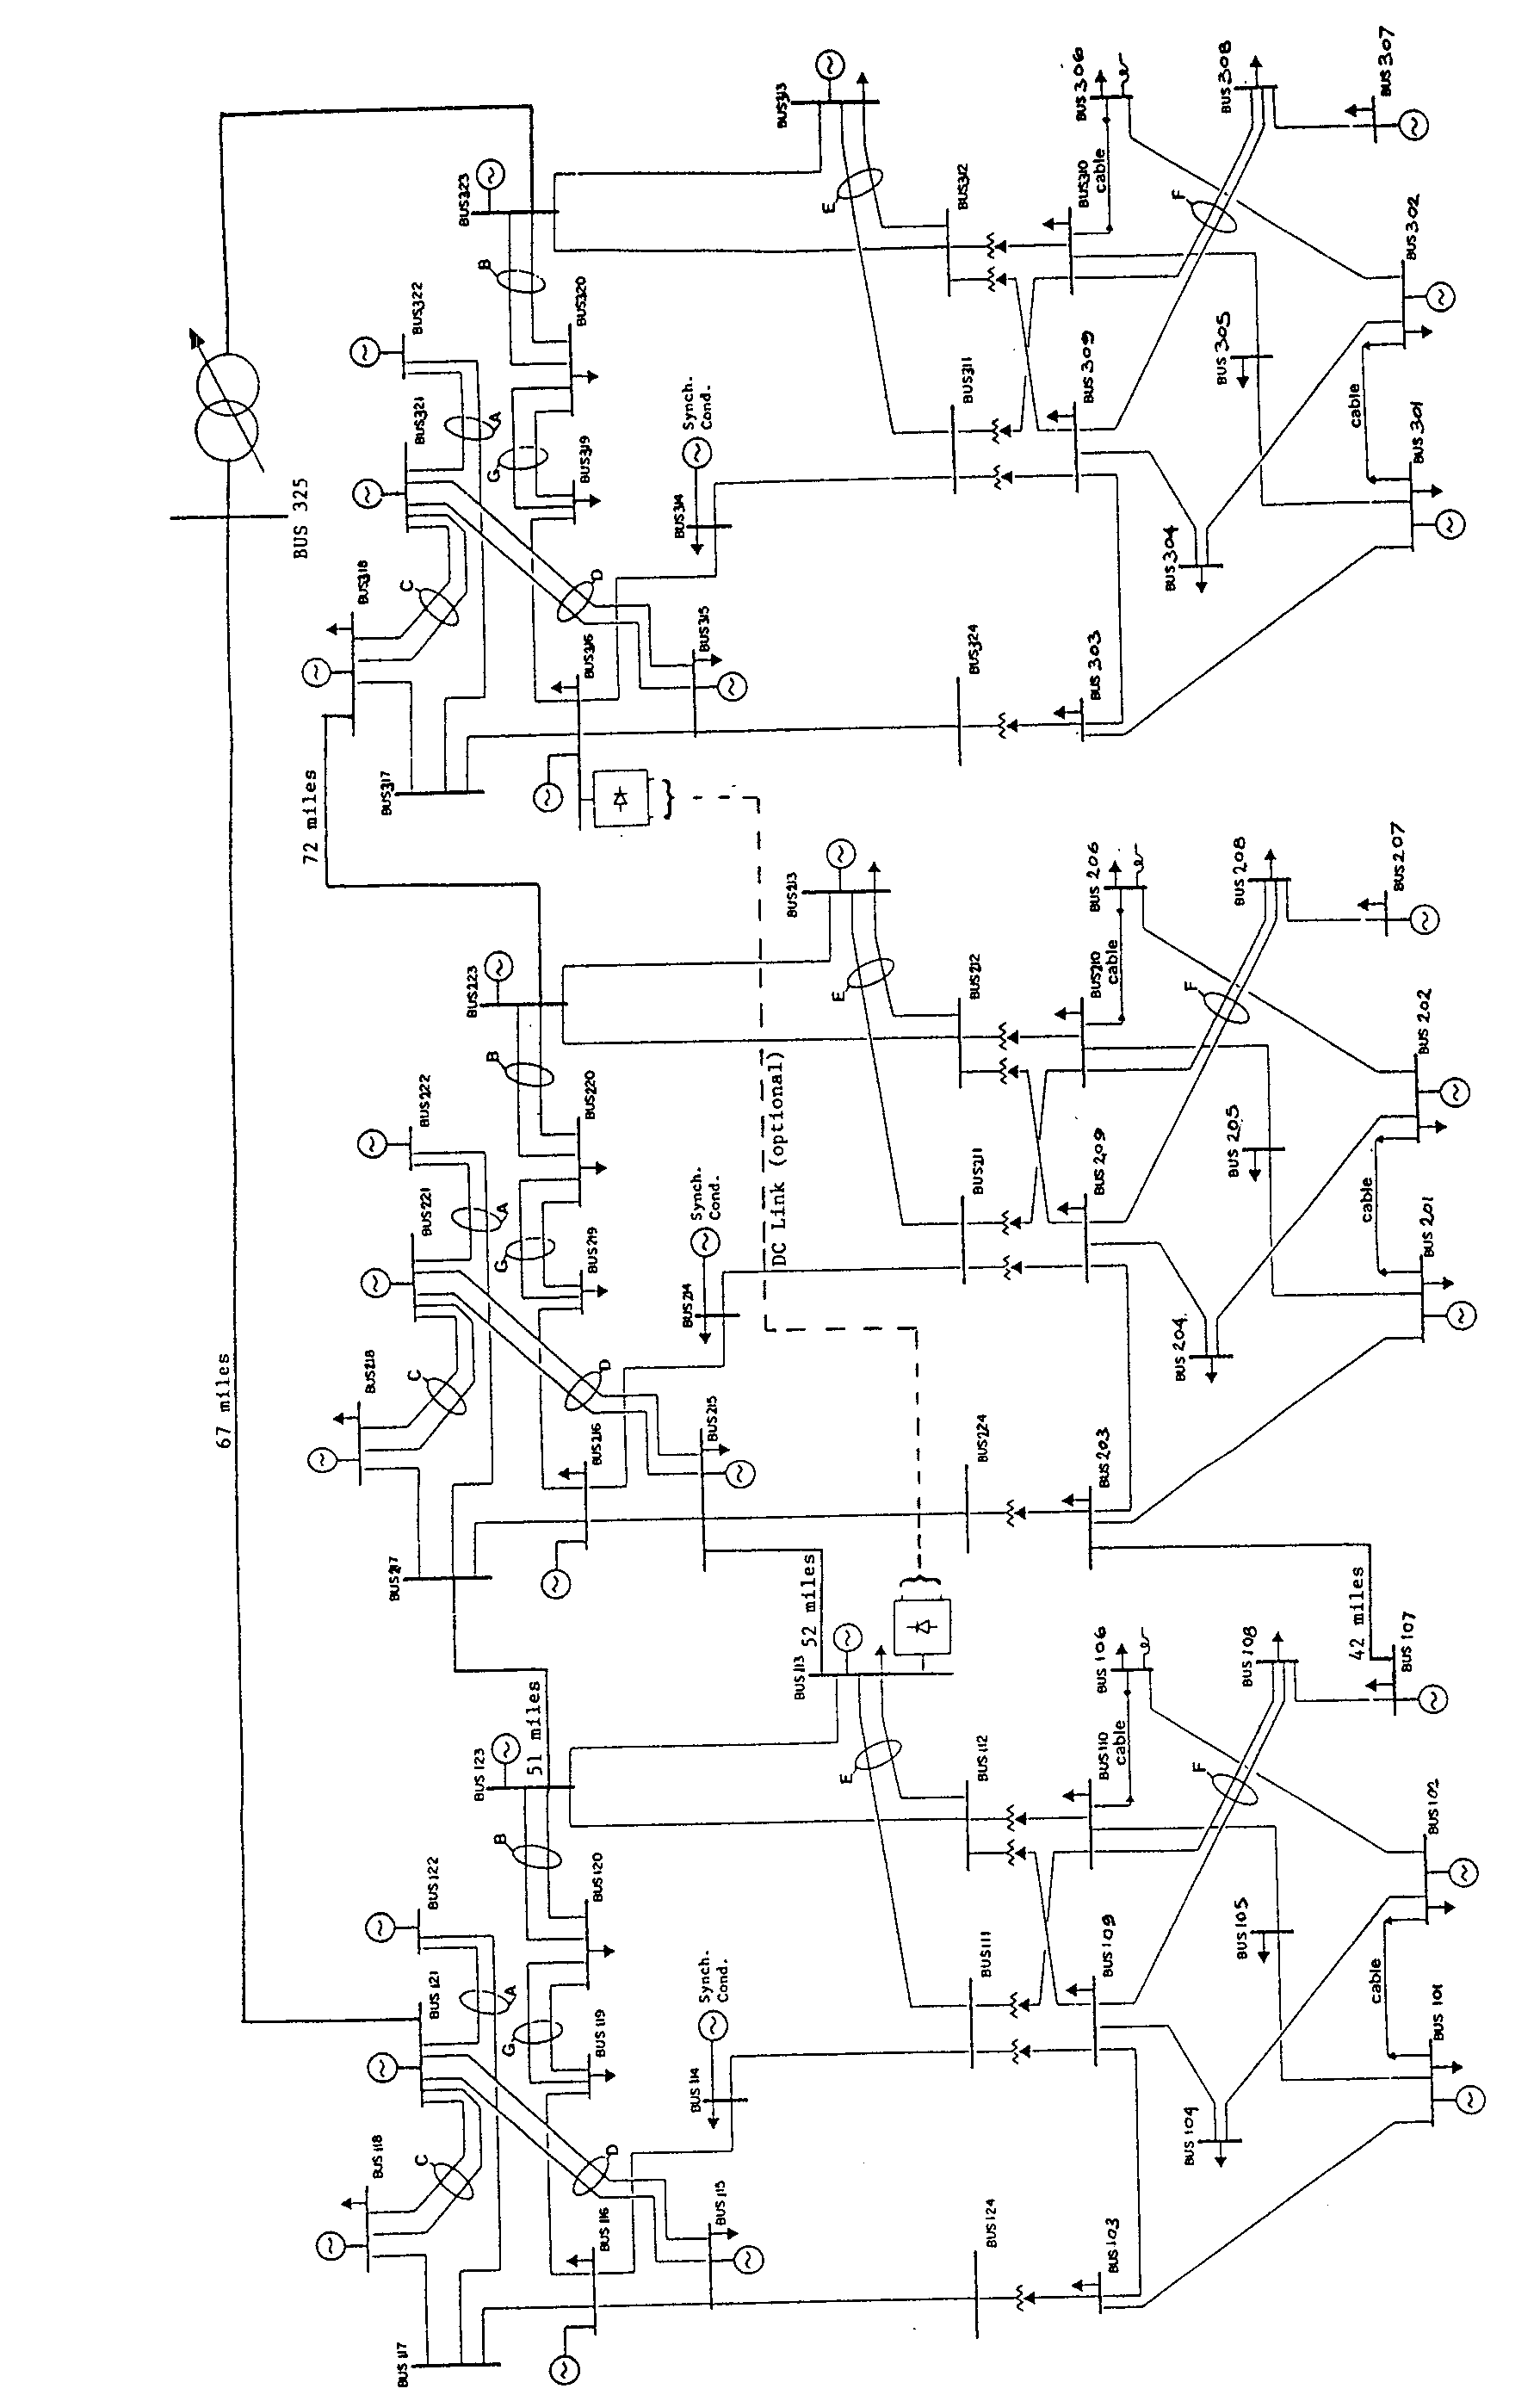
\includegraphics[width=\textwidth,height=\textheight,keepaspectratio]{ieeetopology.png}
  \caption{RTS-96 topology \cite{wongieee}}
  \label{fig:ieeetopology}
\end{figure}

The dataset describes a peak load for each bus. The absolute load in every hour is a percentage of the peak load based on 3 components: the week year, the day of week an the hour of the day. The hourly peak changes according to the season and if it is in a weekend or not. For example, the peak load of bus 101 is 108MW. On 01/07 at 12:00 PM the load is:

\begin{multline}
L_{b = 108} =  (L_{yearweek = 27} = 75.5\%) \times (L_{dayofweek = friday} = 94\%) 
\\ \times (L_{hour= 12 PM} = 93\%) \times 108 = 71.28MW
\end{multline}

Figure \ref{fig:totalSystemLoadJuly} displays the total system load throughout the month of July.

\begin{figure}[h] 
  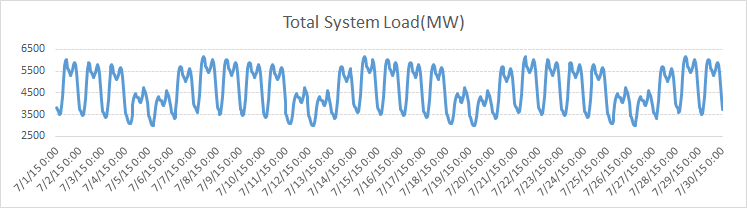
\includegraphics[width=\textwidth,keepaspectratio]{totalSystemLoadJuly.png}
  \caption{Total system load (MW) in July 2015}
  \label{fig:totalSystemLoadJuly}
\end{figure}

To generate instances with sub-hourly load profiles, the load during intra-hour periods is constructed using linear interpolation plus an additional perturbation, which follows a uniform $[-Pr,+Pr]\%$, where $Pr$ is a parameter in the range of [0,100] \%. The objective is to capture the ramping behaviour of NVRE on a sub hourly level. Figure \ref{fig:perturbationDifference} shows a difference between load curve on a 60-minute and 15-minute planning level. 

\begin{figure}[h] 
  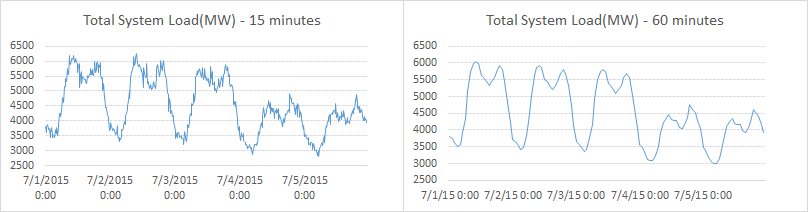
\includegraphics[keepaspectratio]{perturbationDifference.png}
  \caption{System load (MW) for 5 days in July with 15- and 60-minute resolution.}
  \label{fig:perturbationDifference}
\end{figure}

The original RTS-96 system has 87 generators distributed across the test field, with the distribution described in figure \ref{fig:generatorDistribution}. Sync generators are not considered for this study.

\begin{figure}[h!] 
  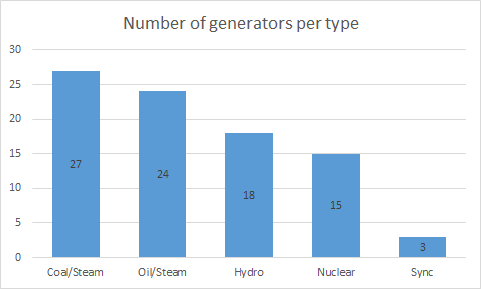
\includegraphics[width=\textwidth,keepaspectratio]{numberGeneratorsPerType.png}
  \caption{Total number of generators per type.}
  \label{fig:generatorDistribution}
\end{figure}



The total peak load is 8550 MW while the total generation capacity is 9975 MW. 

\subsection{Renewable Generators Data}

Although RTS-96 has most of the necessary data for this project, it does not contain any wind and solar generation information, the two fastest growing renewable sources in the world. This discrepancy is interesting in its own right as it reveals how much technology has changed in the two decades since the RTS-96 data set was published.

Since wind and solar energy are expected to play a prominent role in the future grid (e.g., India has pledged to install 100 GW of solar capacity by 2022 \cite{mitindia}, while Germany has already installed 45 GW of wind capacity or roughly 25 \% of its total installed capacity\cite{fraunpower}, wind and solar profiles were also included in our test instances. Historical data for both sources was taken from the website of the Electric Reliability Council of Texas (ERCOT), the independent system operator that manages the flow of electric grid for the vast majority of Texas.  

The wind and solar profiles defines the generation capacity for these renewable resources in a full year, and it is based on historical availability from the last 5 years in Texas. The geographic renewable potential in Texas were considered for each bus in the system, both for solar and wind generators.

\subsubsection{Wind Profile}


Figure \ref{fig:texasWindProfile} shows the Texas Annual Average Wind speed and the relative geographic positions of RTS-96 buses \cite{wongieee}. The flat northern border is known as the "panhandle" because the state of Oklahoma, north of Texas, is shaped like a pan. The handle of this pan is where most of the wind potential resides. In result, most of the new generators are being installed in northwest \cite{texasWindProfile}.

\begin{figure}[h!] 
  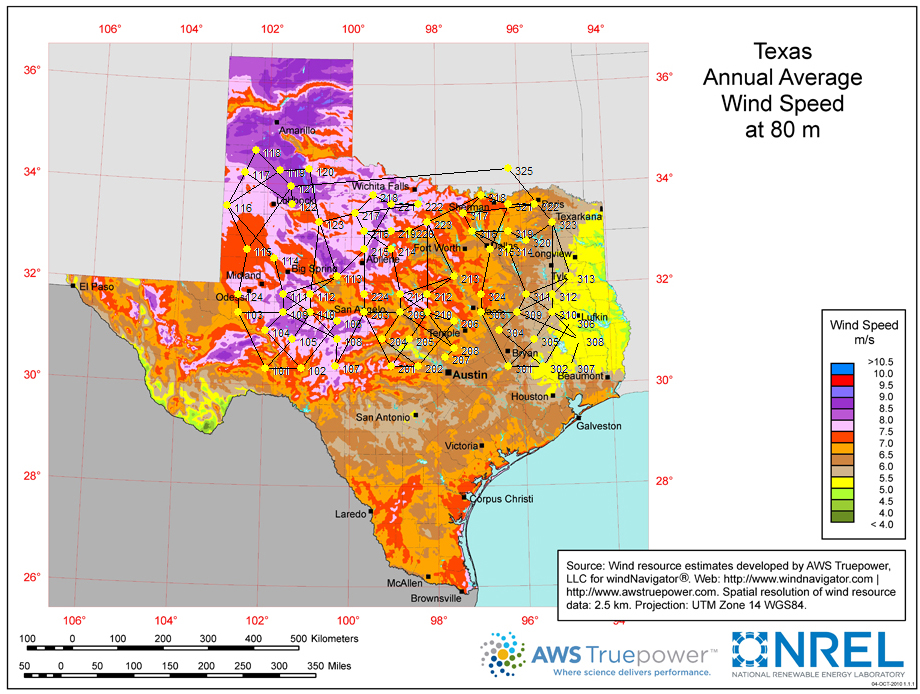
\includegraphics[width=\textwidth,keepaspectratio]{texasWindProfileWithBuses.png}
  \caption{Wind Potential for Texas with RTS-96 Bus Locations. Adapted from \cite{texasWindProfile} }
  \label{fig:texasWindProfile}
\end{figure}


To build the wind potential, each bus was associated with a Texas city or region along with the average historical wind generation for the past 5 years. The studied data is freely shared by ERCOT \cite{ercotGenerationWind}. Therefore each location has a wind potential on an hourly level throughout an entire year. In sub-hourly levels the availability follows the interpolation between the hours followed by a uniform perturbation, using the same logic as load. That said, the real generation for any wind generator is a factor of the percentage of the nameplate capacity followed by the profile where it is located. Figure \ref{fig:windProfileBus122January} shows the wind profile for the bus 122 in the month of January.

\begin{figure}[h!] 
  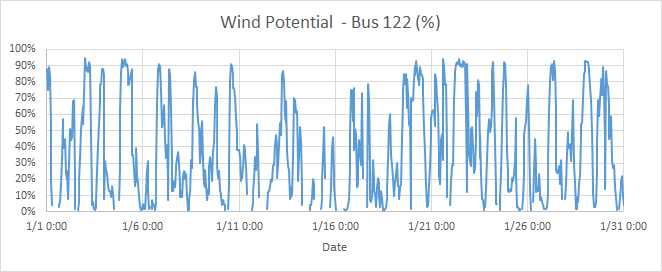
\includegraphics[width=\textwidth,keepaspectratio]{windPotentialBus122.png}
  \caption{Wind Profile for Bus 122 in January}
  \label{fig:windProfileBus122January}
\end{figure}

\subsubsection{Solar Profile}

Figure \ref{fig:texasSolarProfile} displays the NREL's solar incidence report in the state of Texas and the relative geographic positions of RTS-96 buses. 

\begin{figure}[h!] 
	\begin{center}
		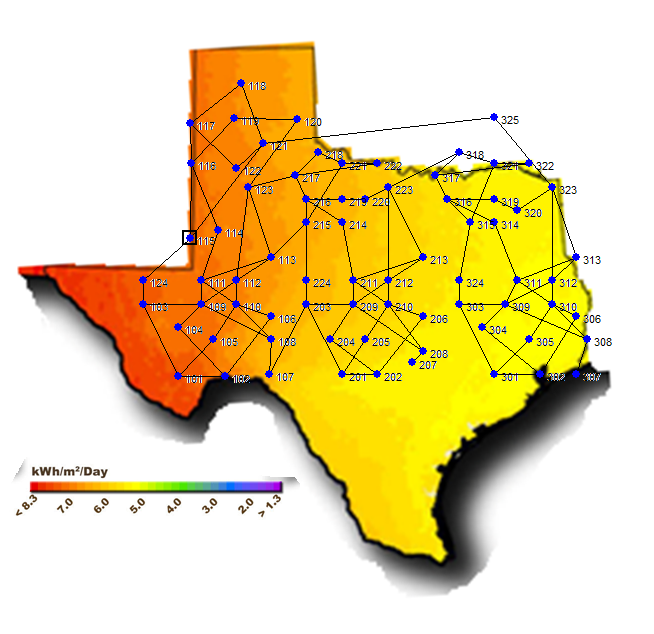
\includegraphics[width=0.6\textwidth,keepaspectratio]{texasSolarProfileWithBuses.png}
	  	\caption{Solar Potential for Texas with RTS-96 Bus Locations. Adapted from \cite{texasSolarProfile} }	  				        \label{fig:texasSolarProfile}
	\end{center}
\end{figure}


It is important to notice that the highest incidence profile in the state of Texas is located in west, followed by northeast and center. The solar profile analysis follows the same logic developed in the wind case. However, only buses located in the mentioned area had their profiles built. As an example, the solar profile for bus 112 (in far northeast of Texas) on January is shown in figure \ref{fig:solarProfileBus112January}.

\begin{figure}[h!] 
	\begin{center}
		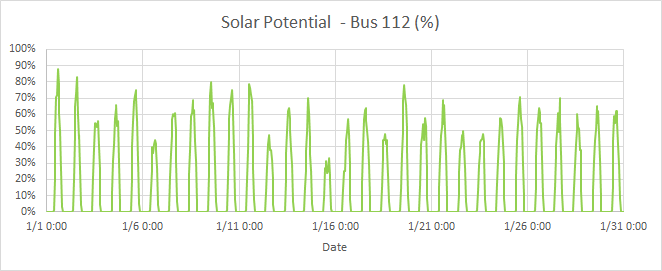
\includegraphics[width=0.8\textwidth,keepaspectratio]{solarPotentialBus112.png}
	  	\caption{Solar Profile for Bus 112 in January }
     	\label{fig:solarProfileBus112January}
	\end{center}
\end{figure}


\subsection{Costs}

For our models, the costs were developed based on the RTS-96 data and some benchmarket values widely used in the industry for power generation studies. There are two type of costs associated with generation:

\begin{itemize}
\item Generation Cost ($\$/MW$): Cost to generate 1MW of a specific unit group.
\item Start-up Cost ($\$/MW$): Cost to change the state of a specific generator type from off to on.
\end{itemize}

\subsection{Scenarios Description}

This project covered 3 different generators scenarios in the same load profile. The distribution is adapted from \citeauthor{shavel} \cite{shavel}, that describes the technical and economical potentials of exploring natural gas and VRE in the state of Texas \cite{shavel}. 

\subsubsection{Scenario 1: Reference}

This scenario captures the existing ERCOT capacity mix. 88\% of generation comes from non-renewable energy sources. The remaining capacity is filled by wind generators, located in the buses that has the Texas Northwest's wind potential (Buses 111-124).

\subsubsection{Scenario 2: Stronger Federal Carbon Rule}

Scenario 2 is build based on column "2032 Total" of table IV-10 in \cite{shavel}. This scenario is described as follows:

\begin{quotation}
"Our scenario with a strong federal carbon rule requires existing coal plants to capture and sequester 90\% of their CO2 output.(...)
As one would expect, this case shows that most of the ERCOT coal plant fleet retires in 2025, the year we assume the carbon rule goes into effect. At this point, 16 GW of coal capacity providing more than 30\% of all ERCOT energy rapidly shifts to gas and renewable supply sources: 6 GW of new CC capacity and 3 GW of new wind capacity. In the next several years, another 3 GW of CC capacity is added, along with another 19 GW of wind. Solar becomes rapidly cost-effective in this scenario and quickly rises to over 8 GW installed by 2029. For the remainder of the scenario horizon, all additional load growth is met by solar and wind additions.”
\end{quotation}

In essence, 44\% of the generation is provided by natural gases, followed by 42\% of NVRE and 14\% of other sources. Most of the wind generators are located at buses 111-124, with some in 211-224. Solar generators are at buses 101-110.


\subsubsection{Scenario 3: "Almost Green World"}

This scenario is an extreme case of Scenario 2. All coal, nuclear and oil/steam generators have been retired and are no longer a part of the system. The grid runs entirely on wind and solar, with advanced natural gas combined cycle generators used primarily for ramping, flexibiliy and backup, i.e, to complete the demand whether there is not enough wind and solar to fulfil the load. Wind and solar generators are located throughout the map, following the concentration based on wind and solar profiles from figures \ref{fig:texasSolarProfile} and \ref{fig:texasWindProfile}.

\subsubsection{Scenario 4: "Green World"}

In this scenario all the natural gases are replaced by battery storage. The generation is 100\% provided by wind and solar generators, with nameplate capacity bigger than Scenario 3. To mitigate the transmission generation limits, wind generators are located all over the field, while solar generators are still located in north east. There is no decision to turn on and off any generator, and the main decision is only how the storage behaviours in order to minimize under generation.

\subsubsection{Generation per Scenario}

The nameplate capacity of base case scenario described by \citeauthor{shavel} \cite{shavel} is 82,949 MW, where for RTS-96 is close to 10,000 MW. Therefore all absolute generator type capacities were adapted to the new baseline and the rates by type were mantained. The result is in Table \ref{table:ScenarioDataDescription}.

\begin{table}[h]
\centering
\caption{Capacity of each generator type expressed in MW as a percentage of total capacity in the 4 scenarios}
\label{my-label}
\begin{tabular}{|lllllll|l|l|}
\hline
               & \multicolumn{2}{l}{\textbf{Scenario 1}} & \multicolumn{2}{l}{\textbf{Scenario 2}} & \multicolumn{2}{l|}{\textbf{Scenario 3}} & \multicolumn{2}{l|}{\textbf{Scenario 4}} \\ \hline
               & \textbf{MW}         & \textbf{\%}       & \textbf{MW}         & \textbf{\%}       & \textbf{MW}          & \textbf{\%}       & \textbf{MW}          & \textbf{\%}       \\ \hline
Nuclear        & 660                 & 6                 & 440                 & 4                 & 0                    & 0                 & 0                    & 0                 \\ \hline
Coal           & 2530                & 23                & 220                 & 2                 & 0                    & 0                 & 0                    & 0                 \\ \hline
Oil/Gas        & 1650                & 15                & 880                 & 8                 & 0                    & 0                 & 0                    & 0                 \\ \hline
NGCC           & 4180                & 38                & 4400                & 40                & 2287                 & 21                & 0                    & 0                 \\ \hline
NGTC           & 2090                & 6                 & 440                 & 4                 & 404                  & 3                 & 0                    & 0                 \\ \hline
Wind           & 660                 & 12                & 3630                & 33                & 7934                 & 60                & 8000                 & 61                \\ \hline
Solar          & 1320                & 0                 & 900                 & 9                 & 2824                 & 16                & 5452                 & 59                \\ \hline
\textbf{Total} & \textbf{11000}      & \textbf{100}      & \textbf{11000}      & \textbf{100}      & \textbf{13452}       & \textbf{100}      & \textbf{17900}       & \textbf{100}      \\ \hline
\end{tabular}
\label{table:ScenarioDataDescription}
\end{table}


\section{Models}

This section describes the Unit Commitment and Economic Dispatch models used in this project

\subsection{Indices and Sets}

\begin{tabular}{ll}

$g \in \mc{G} $& Set of generators\\
$b \in \mc{B} $& Set of buses\\
$sd \in \mc{SD} $& Set of storage devices\\
$g \in \mc{G}^{NR} $& Subset of non-renewable generators\\
$g \in \mc{G}^{R} $& Subset of renewable generators \\
$gt \in \mc{GT} $& Set of generator types \\
$u \in \mc{U} $& Set of unit groups \\
$l \in \mc{L} $& Set of transmission lines \\
$rr \in \mc{RR} $& Set of reserve requirements \\
$rp \in \mc{RP} $& Set of reserve products \\
$t \in \mc{T} $& Set of time periods \\
$g \in \mc{G^{b}} $& Set of generators in each bus b \\


\end{tabular}

\subsection{Parameters}

\begin{tabular}{ll}

$D_{b,t} $& Load at bus $b$ in time $t$ \\
$C_{g} $& Generation cost for generator g (\$ / MW) $t$ \\
$S_{g} $& Start-up cost for generator g \\
$R^{up}_{g} $& Ramp up limit for generator g \\
$R^{down}_{g} $& Ramp down limit for generator g \\
$G^{max}_{g} $& Maximum generation capacity for generator g \\
$G^{min}_{g} $& Minimum generation capacity for generator g \\
$T^{min}_{l} $& Minimum transmission of transmission line l \\
$T^{max}_{l} $& Maximum transmission of transmission line l \\
$P^{R}_{g,t} $& Power generation of renewable generator g in time t\\
$U^{up}_{g} $& Minimum uptime of generator g (hours)\\
$U^{down}_{g} $& Minimum downtime of generator g (hours)\\
$ST^{max}_{sd} $& Maximum storage capacity of storage device sd (MW)\\
$ST^{ramp}_{sd} $& Maximum storage capacity of storage device sd (MW)\\

\end{tabular}



\subsection{Variables}

\begin{tabular}{ll}

$P^{NR}_{g,t} $& Power generation of non-renewable generator g in time t (MW)\\
$T_{i,j,t} $& Power transmitted from bus i to bus j in time t (MW)\\
$T^{loss}_{i,j,t} $& Power loss in transmission from bus i to bus j in time t (MW)\\
$S_{g,t} $& On/off status of generator g at time n\\
$S^{on}_{g,t} $& Start-up status of generator g at time n\\
$S^{off}_{g,t} $& Shut-down status of generator g at time n\\
$V^{-}_{b,t} $& Under generation slack variable at each bus b in time t\\
$V^{+}_{b,t} $& Over generation slack variable at each bus b in time t\\
$ST^{max}_{sd,t} $& Amount of energy stored in storage device sd in time t\\
$ST^{charge}_{sd,t} $& Amount of energy charged in device sd in time t\\
$ST^{discharge}_{sd,t} $& Amount of energy discharged in device sd in time t\\

\end{tabular}

\subsection{Models}

The economic dispatch model satisfies the load and transmission requirements at a minimum cost, following operational requirements such as generation, transmission and ramp limits. In this model, we assume that the commitment decisions has been already made. The main objective function of the studied models is to minimize operational costs over the planning horizon, including fuel, start-up, storage and other variable costs.

The types of constraints that manages the optimal dispatching are:

\begin{itemize}
\item \textbf{Load Constraints:} For each time period, the amount of power produced and discharge from storage should be equal to the total load and amount charged into a storage. Alternatively, in a node, this equations also considers the inbound and outbound power transmitted.
\item \textbf{Ramping Constraints:}  Each generator has technical limitations that limits the amount of increase and decrease from one period to next one. This is specially important when there are considerable load and VRE fluctuations in consecutive periods.
\item \textbf{Generator Limit Constraints:} When turned on, each generator must produce within a minimum and maximum power limit, under normal operating conditions.
\item \textbf{Transmission Constraints:} Transfer of power between buses is bounded by the nominal power capacity of the transmission line
\item \textbf{Minimum Reserve Constraints:} These constraints are required to handle the variability and uncertainty of renewable generators. They state that the amount of extra generation must be at least some fraction of generation in that period.
\item \textbf{Storage Constraints:} As well as generators, the charging and discharging rates in storage devices has also technological 


\end{itemize}

\subsubsection{Simple Economic Dispatch Model}

\begin{subequations}\label{model:simple_ED}
\begin{alignat}{4}
\min ~~& \sum_{t \in T}\sum_{g \in G^{NR}} P^{NR}_{g,t} C_{g} + \sum_{t \in T}\sum_{b \in B} V^{-}_{b,t} + \sum_{t \in T}\sum_{b \in B} V^{+}_{b,t} \label{eq:ObjectiveFunction} \\
s.t. ~~~& \sum_{t \in T} P^{NR}_{g,t} + \sum_{t \in T} P^{R}_{g,t} + \sum_{t \in T}V^{-}_{b,t} = \sum_{t \in T} D_{b,t}  + \sum_{t \in T}V^{+}_{b,t}  &~& \forall t \in T  \label{eq:loadBalanceConstraint} \\
& P^{NR}_{g,t} - P^{NR}_{g,t - 1} \leq R^{up}_{g} &~& \forall t \in T, g \in \mc{G}^{NR}\label{eq:rampUpRateConstraint} \\
& P^{NR}_{g,t -1 } - P^{NR}_{g,t} \leq R^{down}_{g} &~& \forall t \in T, g \in \mc{G}^{NR}\label{eq:rampDownRateConstraint} \\
& G^{min}_{g}\leq P^{NR}_{g,t} \leq G^{max}_{g} &~& \forall t \in T, g \in \mc{G}^{NR}\label{eq:generationBounds}
\end{alignat} 
\end{subequations}

The constraint \ref{eq:loadBalanceConstraint} states the energy balance in every time. The constraints \ref{eq:rampDownRateConstraint} and \ref{eq:rampUpRateConstraint} states that every generator has to obey the ramp limits. The constraint \ref{eq:generationBounds} states the generation limits for each generator. The use of slack variables $V^{-}_{b,t}$ and $V^{+}_{b,t}$ is necessary to always have feasible solutions, and it is important for scenarios where there is a huge renewable penetrations, when there's an abrupt variation of generation and there is a over or under generation.   

\subsubsection{Economic Dispatch with Transmission Constraints}

In this case, the model has to consider transmission limits and losses, without transmission costs associated. The objective function \ref{eq:ObjectiveFunction} remains the same, and the constraints \ref{eq:rampUpRateConstraint}, \ref{eq:rampDownRateConstraint} and \ref{eq:generationBounds} are als used. The constraint \ref{eq:loadBalanceConstraint} is replaced by  

\begin{subequations}\label{model:edTransmissionConstraints}
\begin{alignat}{4}
&\sum_{g \in G^{b}} P^{NR}_{g,t} + \sum_{g \in G^{b}} P^{R}_{g,t} + \sum_{b^{in} \in B} T_{b^{in},b,t} + V^{-}_{b,t} = D_{b,t}  + V^{+}_{b,t} + \sum_{b^{out} \in B} T_{b,b^{out},t}  &~& \forall b \in B, t \in t \label{eq:transmissionBalanceConstraint} \\
& T^{min}_{l} \leq T_{b^{in},b^{out},t} \leq T^{max}_{l}  &~& \forall b \in B, t \in t \label{eq:transmissionLimits}
\end{alignat} 
\end{subequations}

Constraint \ref{eq:transmissionBalanceConstraint} guarantees that the energy balance is always satisfied for every bus: everything that is generated and received from other buses should be equal to what is loaded and sent throughout the line with the respective losses. If this balance is not satisfied then it is represented in the slack variables . The constraint \ref{eq:transmissionLimits} defines the transmission bounds for each line.

\subsubsection{Economic dispatch model with unit commitment constraints}
Unit commitment is the decision of consider the sets of generators that are turned on and off for the planned time horizon. The model includes decision variables to capture ``on'' and ``off'' states for thermal generators in each time period,along with the start-up and shut-down decisions. \citep{palmintier}. The set of constraints are added to the previous model, and the binary nature of the variables makes the problem an MIP, naturally harder to solve computationally \cite{james}. 

\begin{subequations}\label{model:ucConstraints}
\begin{alignat}{4}
& S_{g,t} = S^{on}_{g,t} - S^{off}_{g,t} + S_{g,t}  &~& \forall g \in \mc{G}^{NR} , t \in \mc{T} \label{eq:logconst}\end{alignat} 
\end{subequations}

Constraint \ref{eq:logconst} specifies the logical condition between the binary variables, assuring that a generator can not be on if it was not turned on. The same is valid for turning it off. Constraints \ref{eq:mindownt} and \ref{eq:minupt} forces the generator to follow their minimum downtime and uptime periods when they are turned on or off. 

When there is the decision of turning the generator on or off, ramping and transmitting only apply if the generator is on in a certain time period. Therefore these constraints has the corresponding binary variable, as shown in \ref{model:UC_NewConstraints}.

\begin{subequations}\label{model:UC_NewConstraints}
\begin{alignat}{4}
& P^{NR}_{g,t} - P^{NR}_{g,t - 1} \leq R^{up}_{g} S_{g,t} &~& \forall t \in T, g \in \mc{G}^{NR}\label{eq:UCrampUpRateConstraint} \\
& P^{NR}_{g,t -1 } - P^{NR}_{g,t} \leq R^{down}_{g} S_{g,t} &~& \forall t \in T, g \in \mc{G}^{NR}\label{eq:UCrampDownRateConstraint} \\
& G^{min}_{g} S_{g,t}\leq P^{NR}_{g,t} \leq G^{max}_{g} S_{g,t} &~& \forall t \in T, g \in \mc{G}^{NR}\label{eq:UCgenerationBounds}
\end{alignat} 
\end{subequations}
 
It is important to highlight that if a generator is down in previous period so it can reaches the minimum generation level in the period it is on; otherwise it can not exceed the ramping rate <make it better here>

In unit commitment model, each generator must satisfy a minimum period to remain on or off whether there is a state change on a certain period. Down time constraints are  useful to keep maintenance of a generating unit once has been shut down. Uptime constraints are useful to guarantee stability and to reduce equipment degradation. 

\begin{subequations}\label{model:ucMinDownUpConstraints}
\begin{alignat}{4}
& \sum_{i = t}^{t + U^{up}_{g} - 1} S_{g,t} \geq S^{on}_{g,i} U^{up}_{g} &~& \forall g \in \mc{G}^{NR}, t \in \mc{T} \label{eq:mindownt} \\
& \sum_{i = t}^{t + U^{down}_{g} - 1} (1 -S_{g,t}) \geq S^{off}_{g,i} U^{down}_{g} &~& \forall g \in \mc{G}^{NR}, t \in \mc{T} \label{eq:minupt}
\end{alignat} 
\end{subequations}

\subsubsection{Economic Dispatch/Unit Commitment with Storage Constraints}

Under a scenario where renewable resources are the major source of energy, storage devices are crucial to address fluctuations and uncertainties in generation, so they are an important key to keep the system stable \cite{dwyer}. When storage devices are available in the system, their operations are governed by the following constraints:

\begin{subequations}\label{model:storageConstraints}
\begin{alignat}{4}
& ST^{max}_{sd,t} = ST^{max}_{sd,t - 1} + ST^{charge}_{sd,t} - ST^{discharge}_{sd,t}  &~& \forall sd \in SD, t \in t \label{eq:storageLimits} \\
&  -ST^{ramp} \leq (ST^{charge}_{sd,t} - ST^{charge}_{sd,t-1}) + (ST^{discharge}_{sd,t} - ST^{discharge}_{sd,t-1}) \leq ST^{ramp}  &~& \forall sd \in SD, t \in t \label{eq:storageRamping}
\end{alignat} 
\end{subequations}

The load balance constraint at each bus \ref{eq:transmissionBalanceConstraint} also is modified, by incorporating the storage charging and discharging variables for storage devices located at the specific bus, as defined in equation \ref{eq:transmissionBalanceConstraintStorage}

\begin{subequations}\label{model:edTransmissionConstraints}
\begin{alignat}{4}
&\sum_{g \in G^{b}} P^{NR}_{g,t} + \sum_{g \in G^{b}} P^{R}_{g,t} + \sum_{b^{in} \in B} T_{b^{in},b,t} + V^{-}_{b,t}  + ST^{charge}_{sd \in b,t} = D_{b,t}  + V^{+}_{b,t} + \sum_{b^{out} \in B} T_{b,b^{out},t} + ST^{discharge}_{sd \in b,t}  &~& \forall b \in B, t \in t \label{eq:transmissionBalanceConstraintStorage}
\end{alignat} 
\end{subequations}

In the case where there is no transmission constraints, the storage is incorporating in the general balance constraint \ref{eq:loadBalanceConstraint}

\begin{subequations}\label{model:simple_ED}
\begin{alignat}{4}
s.t. ~~~& \sum_{t \in T} P^{NR}_{g,t} + \sum_{t \in T} P^{R}_{g,t} + \sum_{t \in T}V^{-}_{b,t} + \sum_{sd \in \mc{SD}} ST^{discharge}_{sd,t} = \sum_{t \in T} D_{b,t}  + \sum_{t \in T}V^{+}_{b,t} + \sum_{sd \in \mc{SD}} ST^{charge}_{sd,t} &~& \forall t \in T  \label{eq:loadBalanceConstraintStorage}
\end{alignat} 
\end{subequations}

It is important to highlight the difference between storage, reserve and slack variables in the power planning systems world.  \citeauthor{rebours} \cite{rebours} defines reserve as the capacity of generating active power that was still not committed yet during each time period, and it is used mainly to regulate the frequency, improve system stability and security and respond to unexpected events. Storage is the capability to retain the excess of power generated that was not used and can be used afterwards, either to respond to a low demand, an unexpected peak or a power outage from other generators. Both reserve and storage plays an important key the more VREs are present in the power system. Slack variables guarantees the optimal solution even in the case where there is an unbalance between demand and generation, and it is also an important parameters of analysis when wind and solar is available. In simple storage models, where storage capacity is considered infinite, slack variables can indicate bottlenecks in the transmission system, either indicating a failure in transmission of excess power from generator to the storage device or the necessary power from the storage device to a specific load. When transmission constraints is neglected, the over generation slack variable $V^{+}_{b,t}$ is not necessary, once every generation excess is stored for future uses.



\section{Assumptions}

The following assumptions were made in the model and data during the research and development process:

\begin{enumerate}
\item The load profile is deterministic. There is no forecast error and no variability in the hourly levels peak. For sub-hourly levels all the analysis were made assuming a $\pm20\%$ of perturbation
\item In the Economic Dispatch model, the generation is upper bounded only. All generators can produce from 0 up to their maximum capacity
\item All generators are assumed to be on and ready to generate according to their ramping policies.
\item There is no voltage angle constraint in the model.
\item The model covers the DC version of the ED and UC problems, i.e., only active power is the set of study. There is no reactive power in the developed models.
\item A transmission loss of 1 \% per 100 miles is assumed, which is a coarse representation of reality, but can be easily modelled withing a mixed-integer linear program. This percentage was estimated based on the work of \citeauthor{short} \cite{short}.
\item The loads profiles for buses are positively correlated, and are ruled by the hour, day of week, season and day of week type (weekend or not).
\item There following costs are not presented in the models: transmission, maintenance
\item There is no maintenance factors in generators, like MTTR and MTBF, as well as scheduling. All generators are able to produce power 24 hours per day in ED model and if they are turned on in UC. The assumptions are made to transmission lines.
\item The generation cost is linear per MW.
\item Although the reserve requirements of NVRE is described in this thesis, they are not considered in this work. Therefore there is no reserve requirement and capacity for NVRE.
\item The generation of renewable resources are not in the decision variables. The developed models only decides the generation for non-renewable resources. Therefore the generation is considered a deterministic parameter, not a variable in the model.
\item The load profile is the same for every year.
\item The peak load is constant and deterministic. No stochastic factor is considered in this study.
\item Hear rates are assumed constant as a function of power output.
\item For the storage scenarios, it is assumed unlimited storage capacity. Thus all the over generated power is stored for future uses.
\item The storages are assumed to be 100\% efficient, so everything is stored is instantly available to fulfil the load.
\end{enumerate}

\section{Implementation}


\subsection{Software Selection}

During the briefing process, it was necessary to choose the software platform that matches our project goals, such that it allows the development, run an analysis the project feasible time. 3 options were considered:

\subsubsection{MATPOWER}

MATPOWER is a powerfull tool designed to solve AC and DC Power Flow (PF) and Optimal Power Flow (PF) problems. It is an add-on to MATLAB, and is mainly used for education and research, with a small use on industry. \cite{zimmerman} Although \citeauthor{zimmerman} states that is is possible to dispatch the generators on a minimal quadratic or linear cost, it has limitations on committing them, i.e., starting up or shutting down on a multi-period environment. MATPOWER is very powerful on a single time period, but it can provide computational challenges for multi-periods on a larger horizon. Therefore we concluded this tool was not appropriate for this project.

\subsubsection{PLEXOS \textregistered }

PLEXOS \textregistered is a commercial tool to power systems planning, widely used in power industry to energy resources planning and analysis. It provides academic license, although the process is long. One of reasons to not use it was the necessity to use commercial nature of the tool, which could lead to challenges in make everything developed in this thesis available to academic community.  

\subsubsection{AIMMS}


AIMMS is a mathematical programming tool designed to solve optimization problems. It is as powerful as other optimization tools like AMPL, GAMS. Some features include \cite{bisschop}:

\begin{itemize}
\item Easy-to-use design of complex parameters
\item Intuitive representation of calendar and time horizons
\item Set of optimization tools to solve LP, QP, NLP and MINLP problems
\item GUI to build end-user interfaces
\item Open Data Base Connectivity (OBDC) and OLE interfaces, allowing data exchange between most common databases, as Oracle, SQL Server, etc.
\end{itemize}

Due to easiness of use, the fact that an academic license provides 100\% of the tool functionality, and the previous experience of the members of this project, AIMMS was chosen as the supporting tool for this work. The software features are described in next section.

\section{Software Features}

This section briefly cover all the screens and features developed in AIMMS for this project.

\subsubsection{Data Import}

The data import section allows the user to import all the data using the AIMMS specific structure for data text exchange. More details on how prepare the data can be found at \cite{bisschop}.

\begin{figure}[h] 
	\begin{center}
		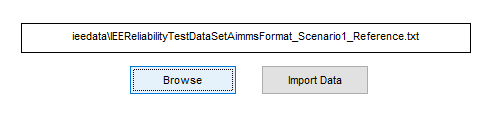
\includegraphics[keepaspectratio]{aimmsScreenImportPage.png}
	  	\caption{Data Import page in AIMMS}
     	\label{fig:aimmsScreenImportPage}
	\end{center}
\end{figure}

\subsubsection{Data Settings}

After the data has been imported, the user has the chance to add/edit and view some data on an intuitive way. In \textit{Network Page}, it is possible to see the location of buses (in yellow), as well as locations of generators per type. The user can change the list to see whatever type he wants. In \textit{Data Buses Page}, it is possible to edit the peak load of each bus in the system. The \textit{Costs Page} has the start-up and variable cost for each generator type and unit group. In \textit{General Data Page} the user can add, edit and remove the main components of the system, i.e., buses, generators and unit groups, as well as changing general configurations, such as horizon dates, granularity and perturbation level for load and wind profiles under a sub-hourly level. 

It is possible also to see the total load over time. In \textit{Generators Specification Page} it is possible to configure the main parameters that defines a generator, such as its type, unit group and bus where it is located. In \textit{Wind and Solar Availability Page} it is possible to view the Wind and Solar profile for the selected bus in the node, as well as locations that have either solar or wind profile mapped (marked with the blue ball). Lastly, the \textit{Summary Page} summarizes the total generation capacity and load, as well as total number of generators and its capacity per generator type.

\begin{figure}[h] 
	\begin{center}
		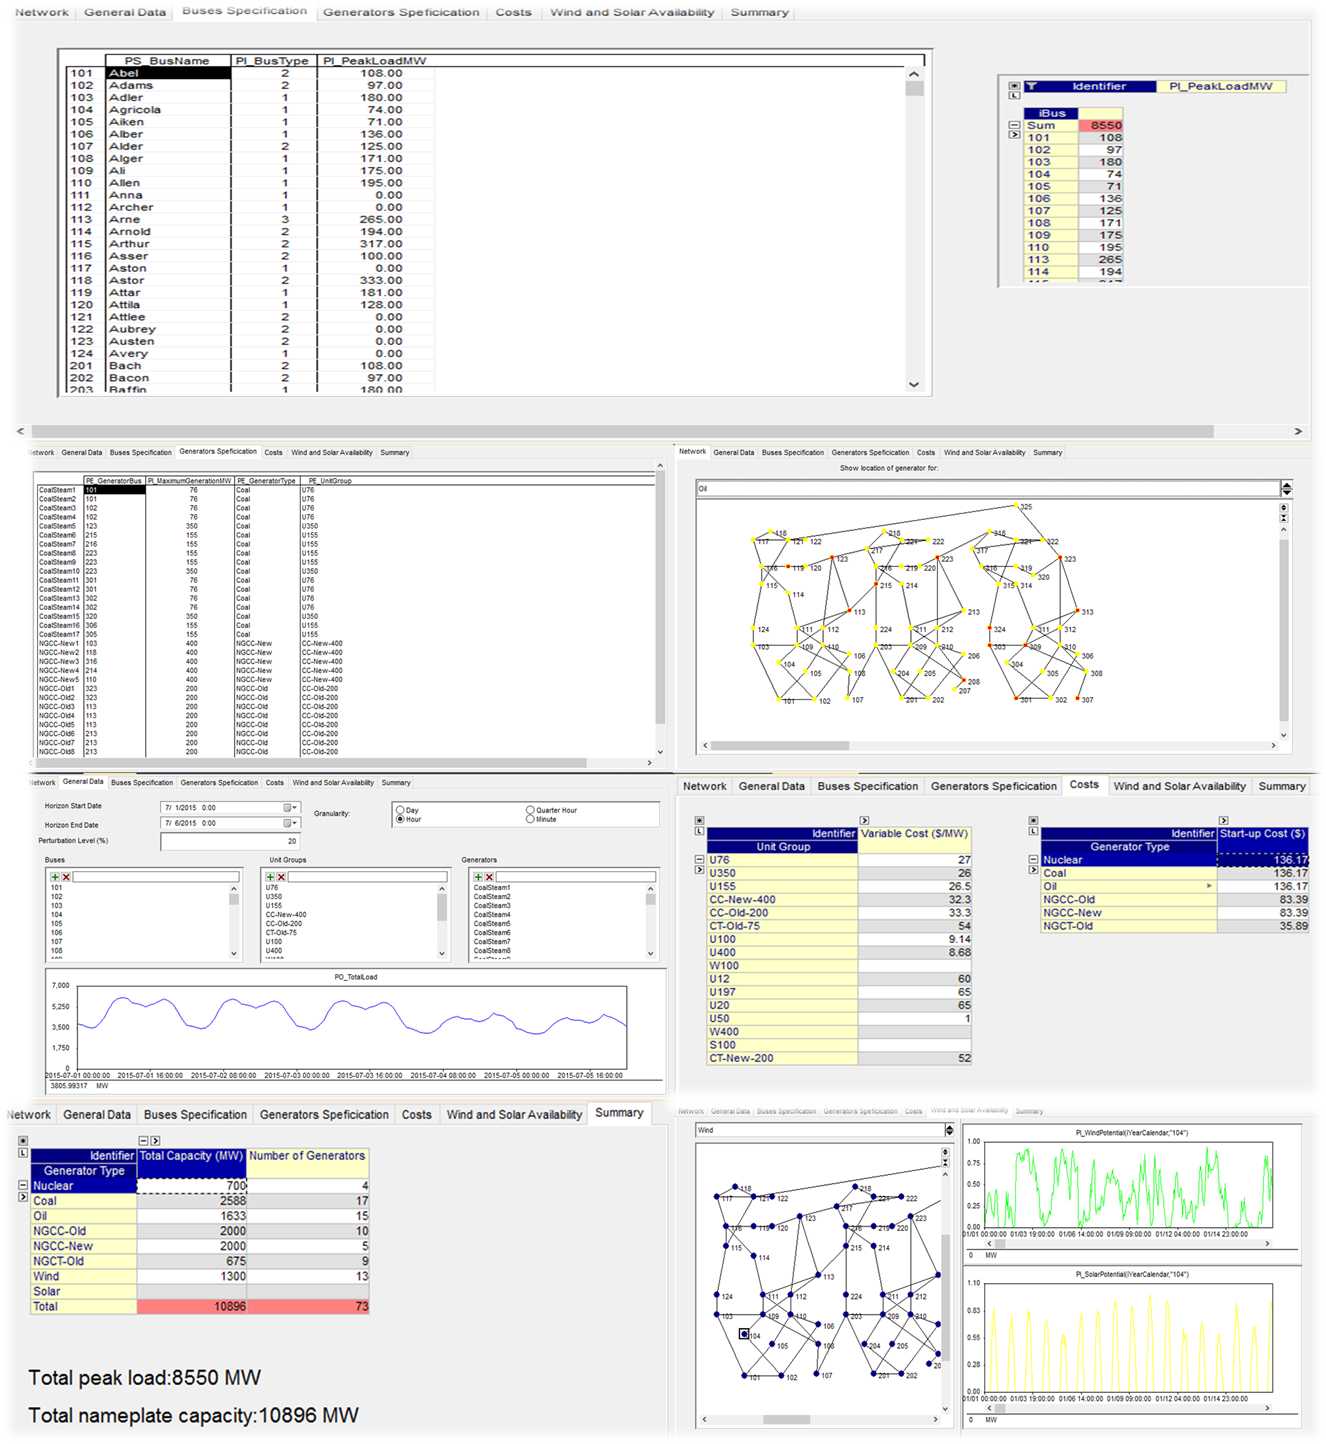
\includegraphics[width=\textwidth,height=\textheight,keepaspectratio]{aimmsDataPages.png}
	  	\caption{Data Section Pages}
     	\label{fig:dataSectionPages}
	\end{center}
\end{figure}


\subsubsection{Optimization and Results}

The optimization section contains all the required settings to run the optimization, as well as the tables and graphs to analyse the results on an intuitive way. 

The user has the option either to solve the Economic Dispatch or Unit Commitment problems, with or without the following features:

\begin{itemize}
\item Ramping Constraints
\item Transmission Constraints
\item Reserve Constraints
\item Slack Variables
\item Transmission Losses (if "Transmission Constraints" is chosen)
\end{itemize}

In \textit{Demand, Load and Transmission}, it is possible to see, for every bus in every time period, the load, generation and transmission flows in and out. It also is possible to see this same flow on a graphic way in \textit{Transmission Map} section, for each time time period, as well as the location of VRE(in green) and active(red) and inactive(gray) NVRE. The \textit{Average Load Distribution} contains the graph displaying the average load for each generator type within a day, while in \textit{Load Distribution Page} it is possible to see the generation distribution per time period, as well as the total load, being useful to identify over and under generation. The \textbf{Power Output Result} details the generation by each generator, in a table. Finally, the \textit{Location Marginal Prices} page contains the Shadow Prices per time for each location, and it is useful to identify potential investments or bottlenecks.

The \textit{Average Ramping} page is useful to compare the ramping behaviour of the generator sources, expressed as:

\begin{equation}
    AverageRamping_{gt \in \mc{GT}} = \overline{\dfrac{P^{NR}_{g,t} - P^{NR}_{g,t-1}}{G^{max}_{g}}}
\end{equation}

In other words, it expresses the average ramping grouped by each generator type , normalized by its maximum capacity. It avoids the misunderstanding of high-capacity generators being ramped more than the lower ones.

\begin{figure}[h] 
	\begin{center}
		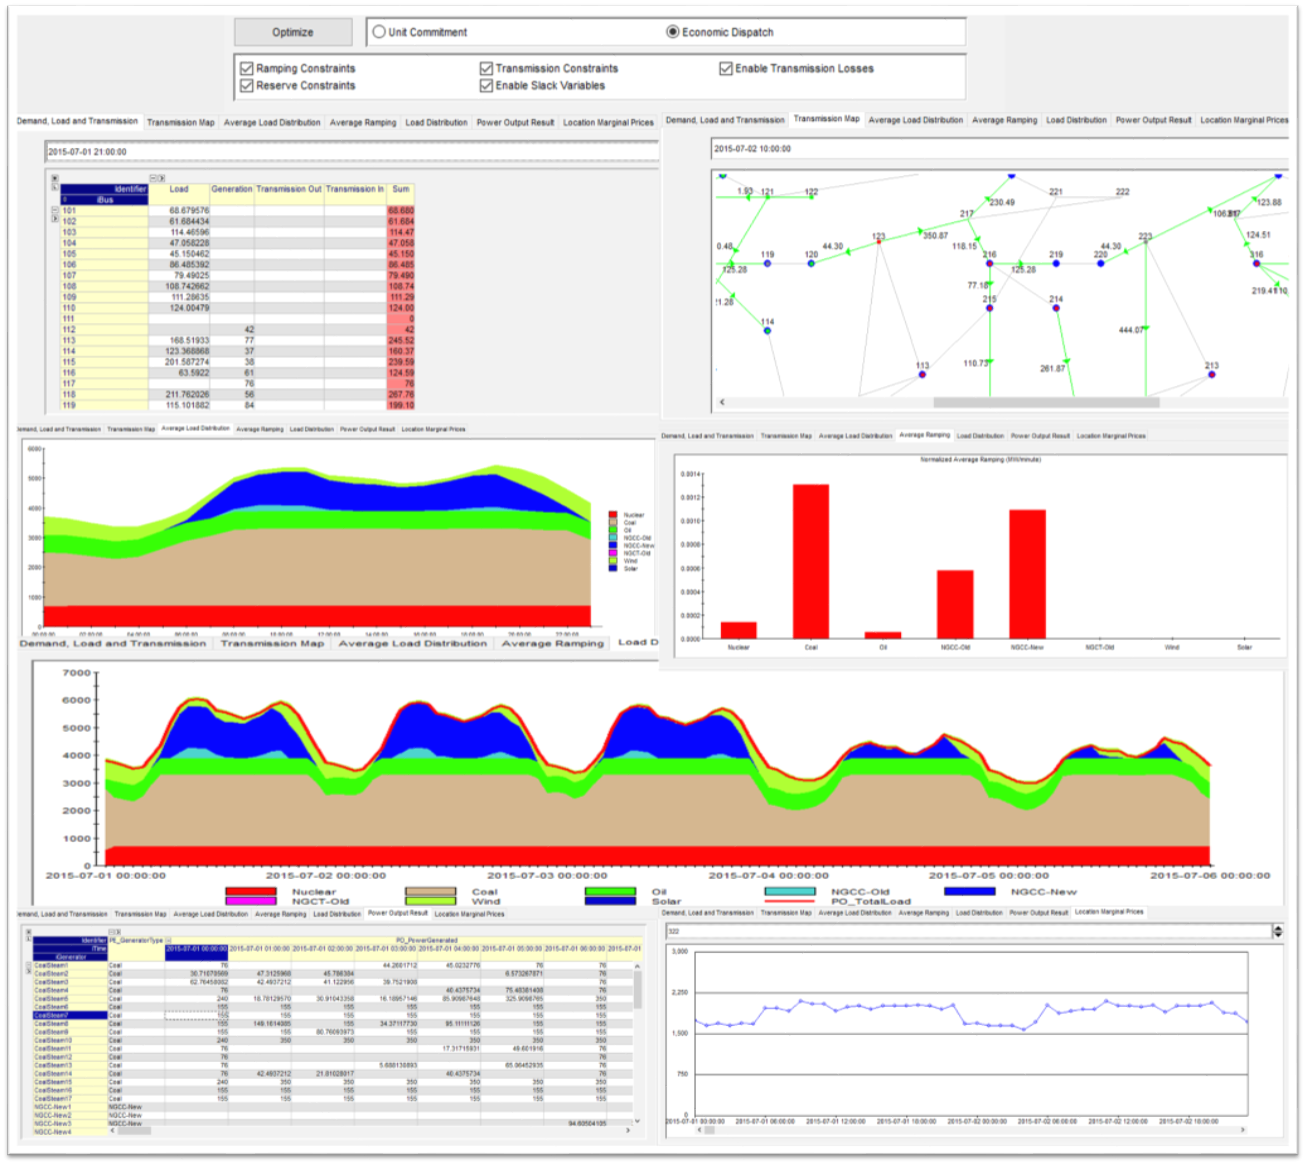
\includegraphics[width=\textwidth,height=\textheight,keepaspectratio]{aimmsOptimizationSectionPages.png}
	  	\caption{Optimization Section Pages}
     	\label{fig:optimizationSectionPages}
	\end{center}
\end{figure}



\chapter{Analysis}

In the analysis make all the scenario runs, describe all the scenarios test, put a table with all the possibilities, and categorize them by model and describe then. Then, make an analysis by ramping, over and under generation, as well as results. Put graphs, tables, everything that supports your points of view.

The analysis has the goal to evaluate the impact of the following components in UC and ED models:

\begin{itemize}
\item Time granularity: 1 hour, 15 minutes and 5 minutes
\item Transmission: with or without transmission
\item Level of VRE: Scenarios 1, 2 and 3
\end{itemize}

With all possible combinations of these factors, there are 36 data sets to analyse. These are defined as "test cases", as described in table Create the Table. The following parameters are object of analysis:

\begin{itemize}
\item Power Output per generation type over time
\item Under and Over Generation over time per bus
\item Running time per test case
\item Ramping distribution for NVRE per generator type
\end{itemize}

\subsection{Power Output per Generation Type}

Figures \ref{fig:powerOutputScenario1}, \ref{fig:powerOutputScenario2} and \ref{fig:powerOutputScenario3} has the power production for each generator type in a combination of model type (UC or ED), granularity (60, 15 and 5 minutes) and transmission constraints on and off. Each figure represents the result for each scenario described in the Data Section. All instances represent the same time period of one week of July, with the same load profile. The generator type colors are described at the bottom of the page, and to make the curve more analysis friendly all the x-axis were removed. There are some interesting analysis, which will be described by Scenario.


When there is no transmission constraints, there was no significant difference of generation distribution between time granularities on the Economic Dispatch version, except for the ramping behaviour of non-renewable resources. It is expected to ramping more due to the variability under a sub-hourly level. 

The generation profile is the same for nuclear, coal and oil sources for the economic dispatch model. When the model is solved with transmission constraints, only NGCC-New generators can not handle the demand under the peak, so they need to be complemented by NGCC-Old ones. The reason for that is the transmission limit on power transmission, wich does not allow NGCC-New generators to fill all the left demand at peak, letting NGCC-New generators supply it.

As for Unit Commitment with Transmission Constraints on a 60-minute level, the NGC-Old generators were turned on during the running process, and remained until the end of the horizon, which reduced the generation of base generators during low demand,specially Nuclear types.

When UC decisions were made on sub-hourly levels, the generation distribution profile differed from the other configurations significantly, which lead to a further investigation. On a 15 minute-level the optimizer decided to turn on most of natural gas generators (NGCC-New, NGCC-Old, NGCT-New) and use NGCT-Old generators to fulfil peak demands, cheaper start-up option than Oil and Coal, and keep few oil generators running at a minimal level. However for the first three days the total demand was not fulfilled during peak load, even for a penalty of \$10000 of MW not generated. We decided then to analyse which constraint was leading to this behaviour, so we disabled the ramping constraints and run the UC model on a 15-minute and 5-minute level. Disabling the constraints augmented the solution space, which could lead to unpractical solution time. Therefore the results has less than 1\% of optimality gap.

The MIP solution took 81 minutes to find a solution with a 0.06\% of the LP Relaxation for the 15-minute level and 300 minutes for a 5-minute. The comparison between Transmission on and Off are shown in \ref{fig:noRampingConstraint}. For both levels, when transmission constraints are not considered, NGCC-Old generators are turned on during peaks, and turned of afterwards. This solution is clearly less practical than turning on most of generators and letting them running at minimal level, and can lead to more maintenance costs.

\begin{figure}[h] 
	\begin{center}
		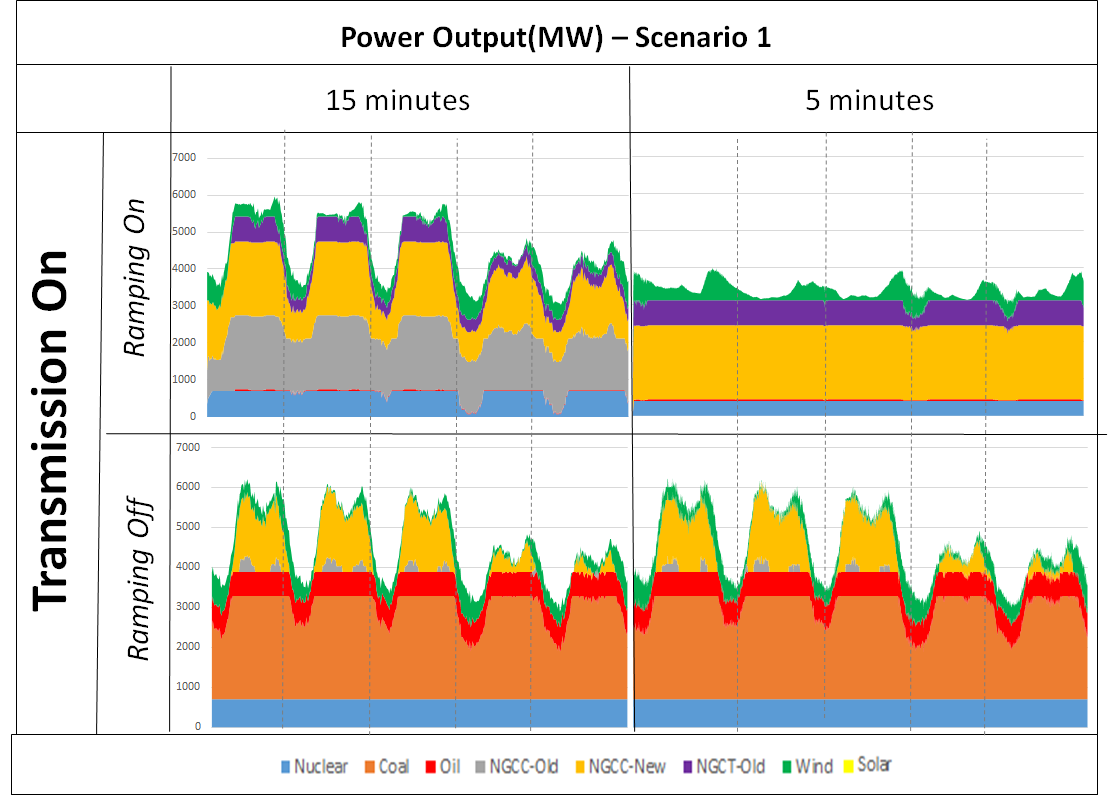
\includegraphics[width=\textwidth,keepaspectratio]{PowerOutputScenario1_NR.png}
	  	\caption{Power Output for Scenario 1 with and without ramping constraints}
     	\label{fig:noRampingConstraint}
	\end{center}
\end{figure}

\begin{figure} 
  \centering
  
	  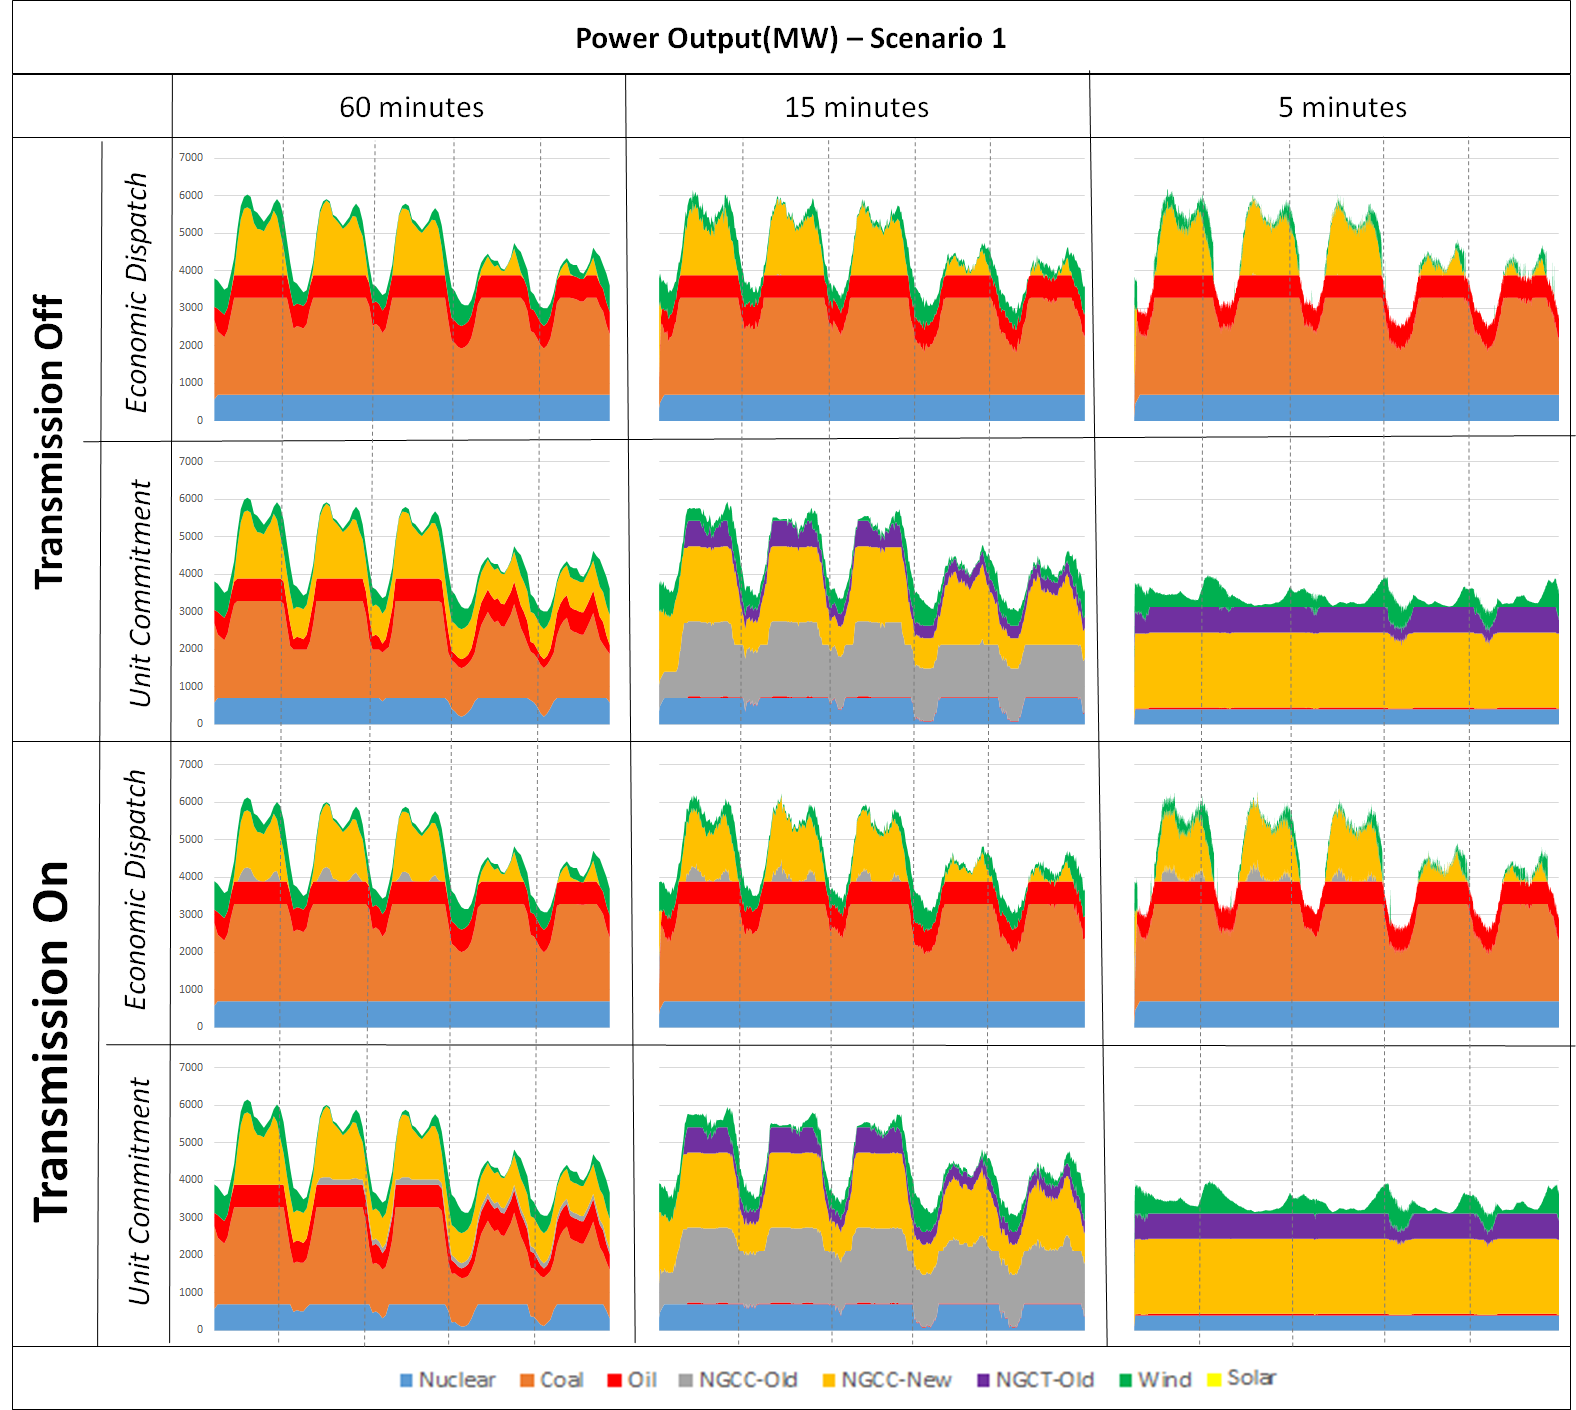
\includegraphics[width=\textwidth,height=\textheight,keepaspectratio]{PowerOutputScenario1.png}
  
  \caption{Power Output for Scenario 1.}
  \label{fig:powerOutputScenario1}
\end{figure}



The Economic Dispatch problems led to some generation distributions for all possible configurations. The similarities of the results between transmission on and off indicates that the transmission limits did not make influence in the final result. 

%This can be seen better Figure **, that displays the utilization per transmission line in the 3 cases of Economic Dispatch versions, and it is easy to see there is no line with high utilization that could be a potential bottleneck.

In the schedules generates by Economic Dispatch, Coal, Oil and Nuclear generator were set to run the whole horizon, where NGCC-New generators were chosen to handle load and wind and solar variabilities across the time. For Unit Commitment the planning of NVRE are different for three time scales. On a 60-minute level, the distribution is almost the same for the Economic Dispatch solutions, but in this case coal and nuclear generators reduce their production when the demand is low and let NGCC-New ones fill the gap. This can lead to increase of maintenance costs because of the ramping behaviour, where in the other hand it strengthen the use of green energy. The fact that the generators has to run under a minimum level and the cheapness of start-up costs for gas generators comparing to oil explains this behaviour difference between Economic Dispatch and Unit Commitment decisions.

%*Generate Image Here.*

Another important aspect to analyse is the UC generation profiles difference between the time scales. Whereas in the 60 minute level Oil, Nuclear and Coal generators are the base of energy, on a 15-minute is  Nuclear only, whereas NGCC-New fill this base while few NGCT-New runs under a minimal level during normal hours, and increases its production during peak hours. 

Under a 15 minute-level more NGCT-Old generators were turned on when transmission limits is ON, caused by the limits of transmitting the energy of NGCC-New generators. Also it was observed the use of few oil generators during peak hours.

\begin{figure} 
  \centering
  
	  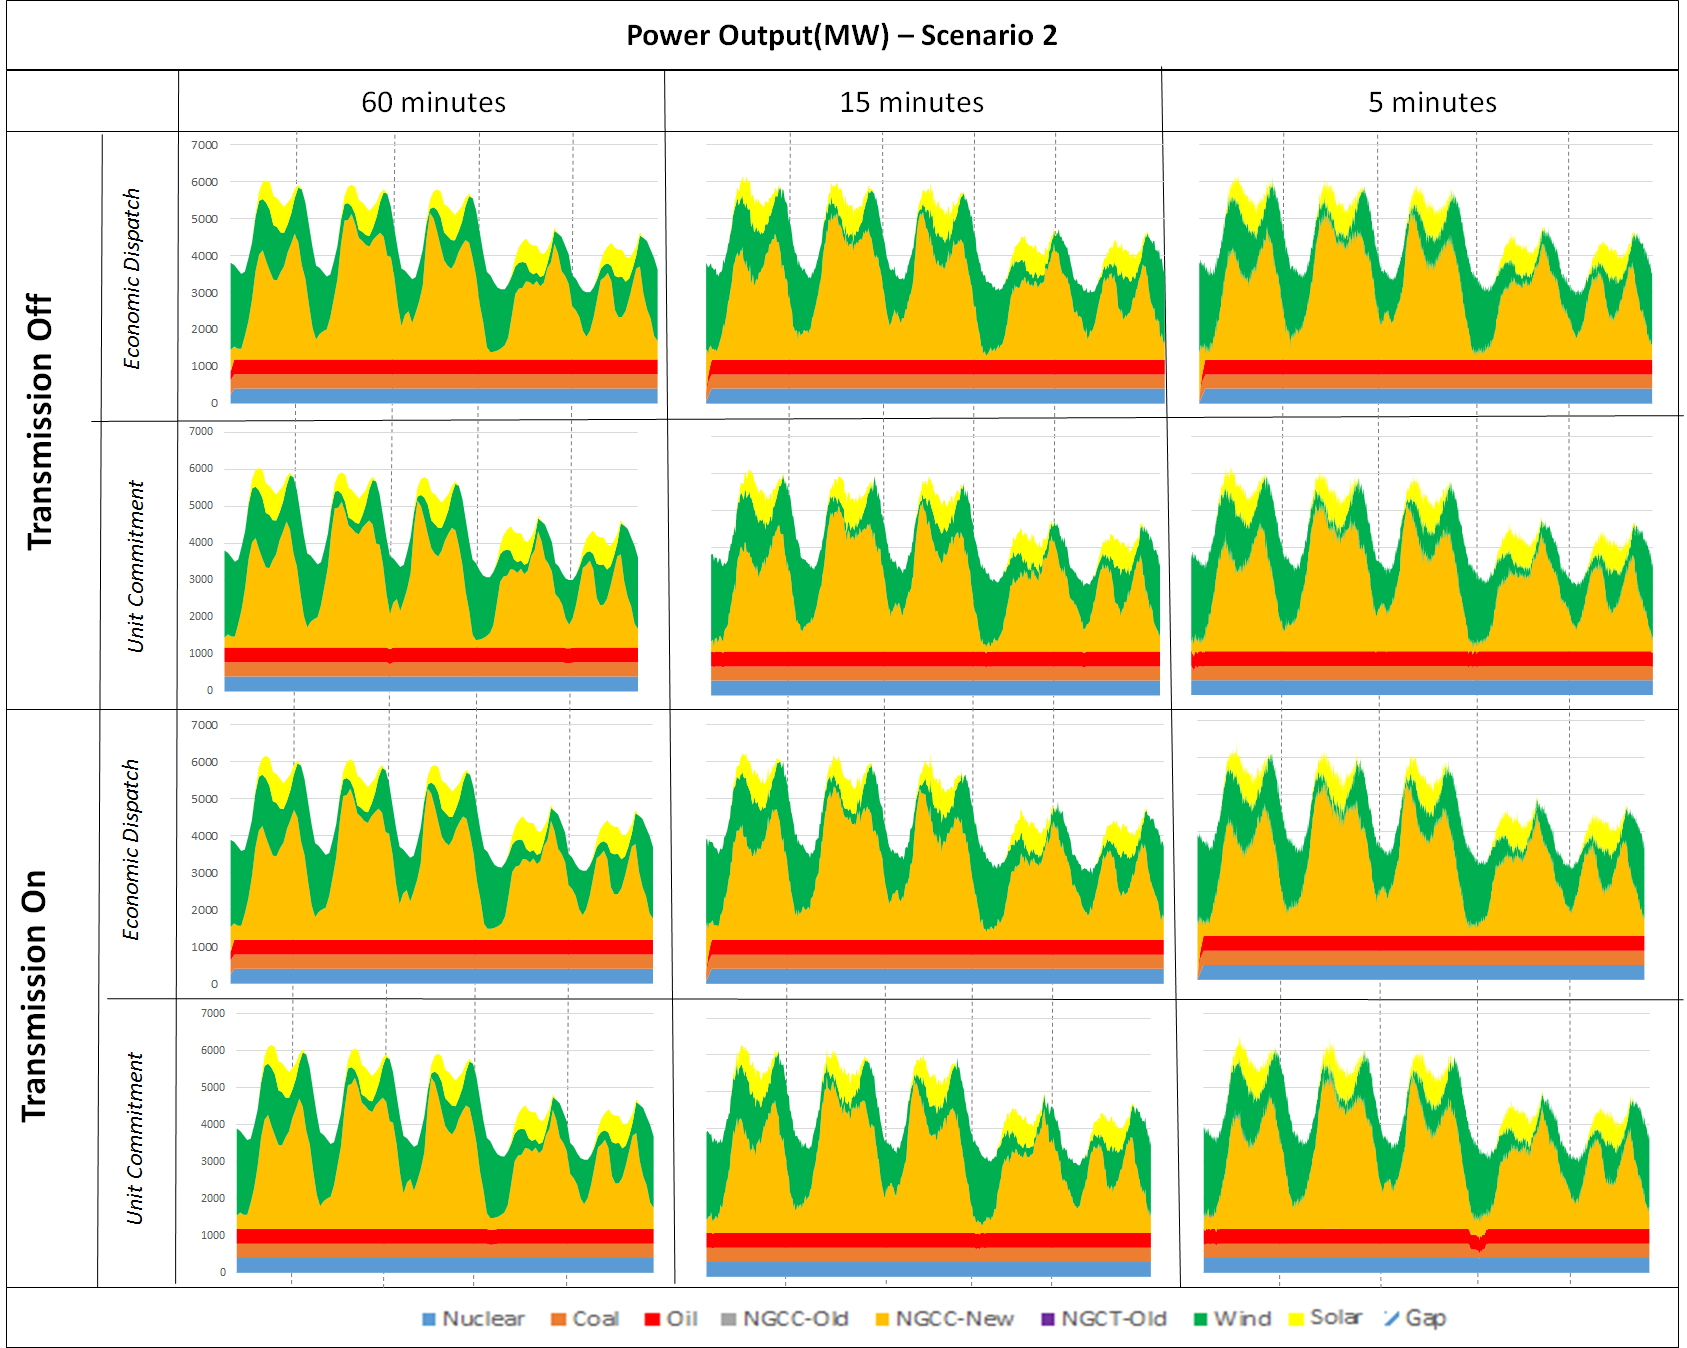
\includegraphics[width=\textwidth,height=\textheight,keepaspectratio]{PowerOutputScenario2.png}
  
  \caption{Power Output for Scenario 2.}
  \label{fig:powerOutputScenario2}
\end{figure}

Scenario 3 perhaps is the most challenging and uncertain set to plan, specially because of high variable resource penetration and their variability over time. In all configurations the demand was not entirely met, specially on peak hours and low wind generation. 

In scenario 3 there is a considerable difference in the generation for non-renewable resources when comparing transmission on and off, for both optimization models. The transmission is a bottleneck in two cases: to fulfil the demand on peak levels and to transmit energy coming from renewable resources. When comparing the generation between UC and ED instances NGCC-New generators are the predominant source of Non-variable renewable energy (NVRE), having NCTG-Old a support to peak and low wind and solar generation moments. The UC decision decided to turn on most of NGCC-Generators and keep them running at a minimal level during low demand when transmission is not consider. For the other case the generation of them is bounded by the line limits, so the solution turns on the generators from other locations. It is easy to see that the ramps are smoother for UC cases, mostly because of the minimum generation levels.

\begin{figure} 
  \centering
  
	  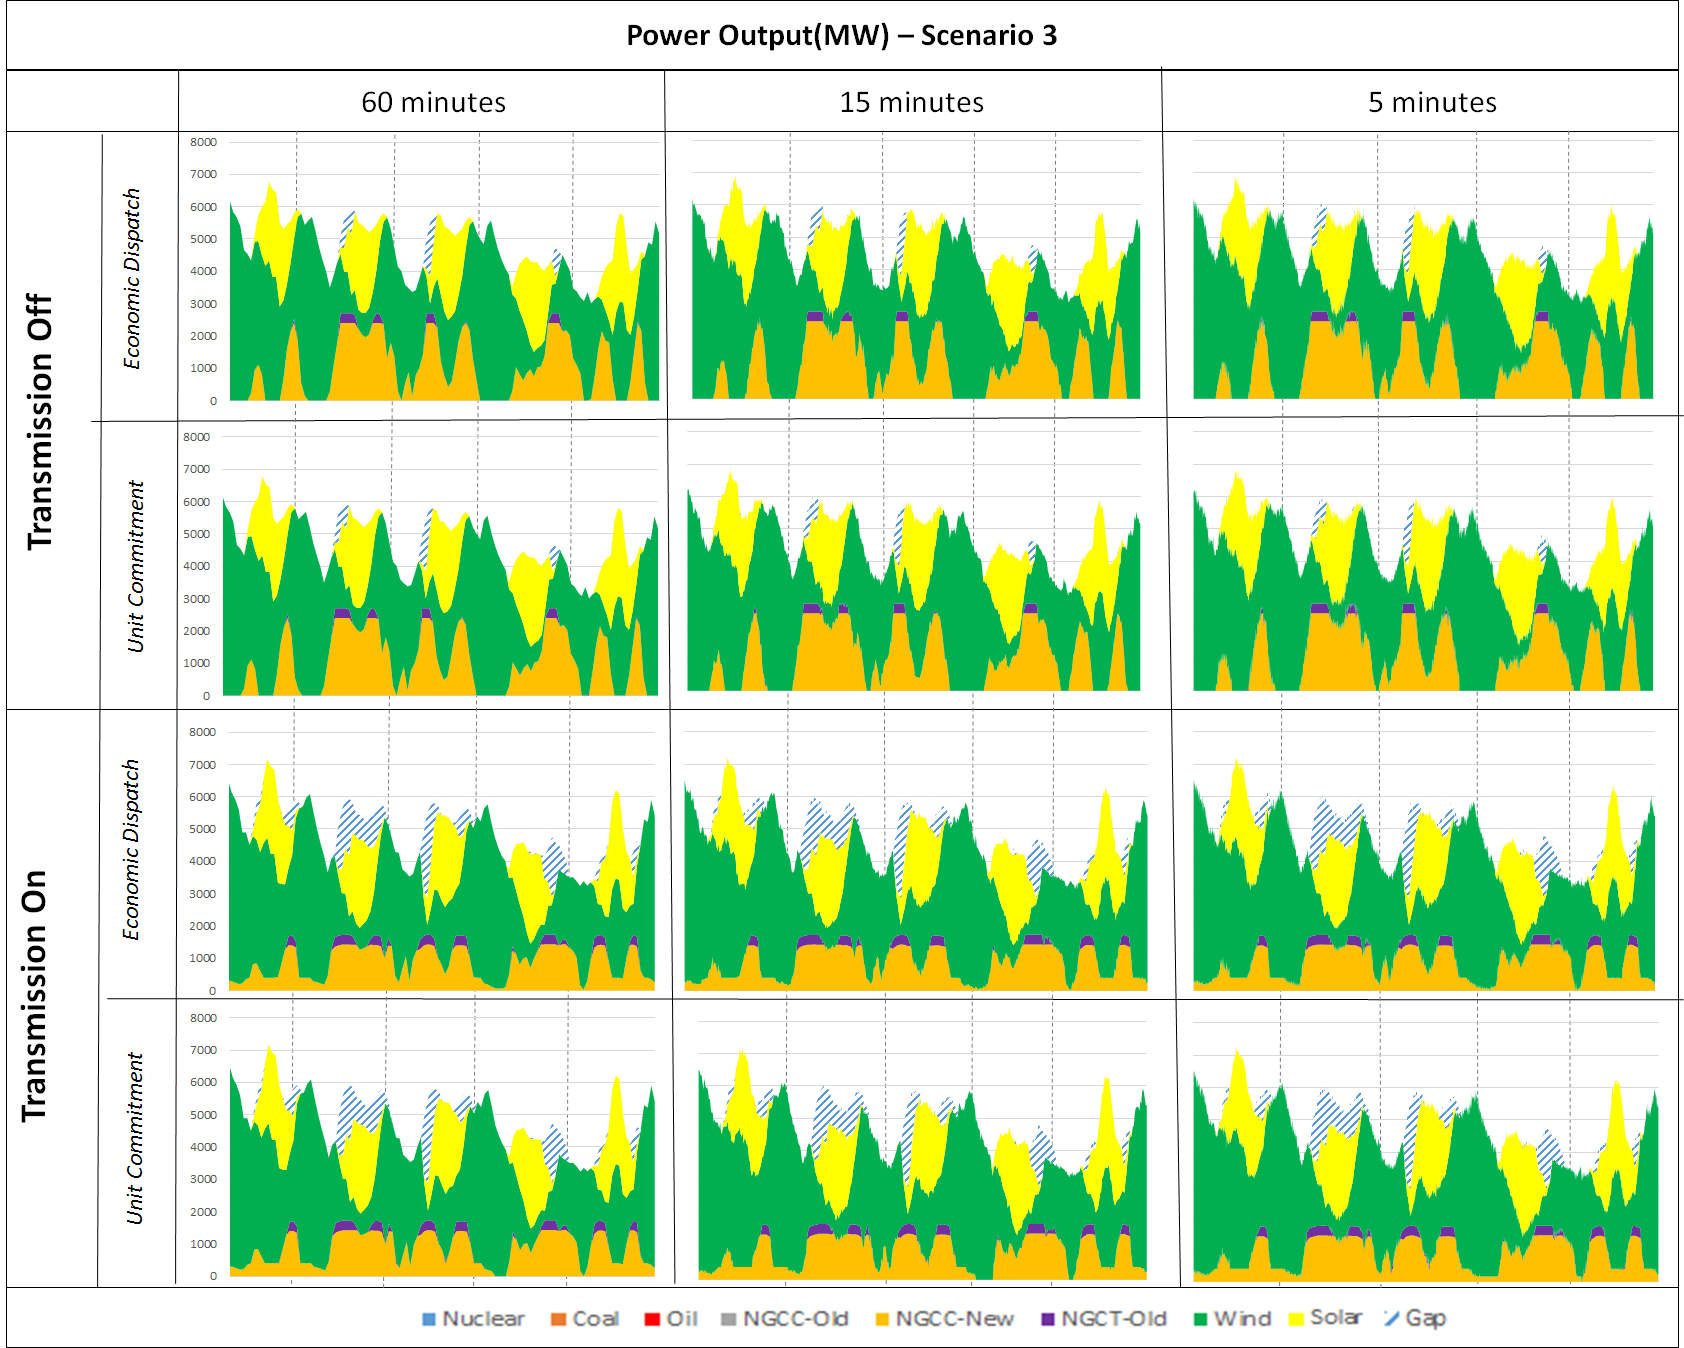
\includegraphics[width=\textwidth,height=\textheight,keepaspectratio]{PowerOutputScenario3.png}
  
  \caption{Power Output for Scenario 3.}
  \label{fig:powerOutputScenario3}
\end{figure}


Two important aspects to evaluate the quality of the optimization result are the final objective function value and the solution time. Figures \ref{fig:solutionparameterss1}, \ref{fig:solutionparameterss2} and \ref{fig:solutionparameterss3} compares these parameters for all the problem instances, per each scenario. The dashed bars represents results out of the y-axis, and their absolute results are in the tables below the graphs. 

In scenario 1, as expected the cheapest and fastest solution were found when no transmission is considered, for 60 minutes level, because of the lower number of variables and constraints. However lower levels with transmission led to faster and cheaper results. In general the solution times for unit commitment are much bigger than economic dispatch instances, due to the MIP NP-Hard nature of the problem. The only exception found was when transmission is off on a 60-minute level, with only 9 of the baseline. The outliers of this curve are represented by dashed bars, and represents UC instances on a sub-hourly level. One can explain the huge values based on the under generation penalties, which was set to 10,000,000 / MW not satisfied. This huge value also could explain why UC instances took so long to solve. Even though, for pratical purposes it is recommended to solve the Unit Commitment on a hourly level.

\begin{figure}[h] 
  \centering
  
	  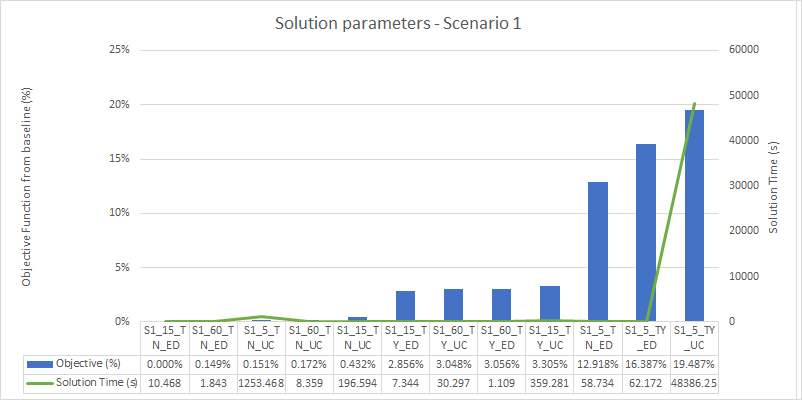
\includegraphics[width=\textwidth,height=\textheight,keepaspectratio]{SolutionParametersS1.png}
  
  \caption{Solution parameters for all instances in Scenario 1. Baseline: $\$658,218,352.9$}
  \label{fig:solutionparameterss1}
\end{figure}

In scenario 2 all the economic dispatch instances generated results close to the baseline. With no transmission all the 3 models generated the same result quality, and the same applies for the ones with transmission activated. However solving the instance on a 5-minute level with transmission was slower than without. The same was observed for unit commitment, and the reason behind that is the expansion of binary solution space when there is no transmission constraints. For sub-hourly levels, the solution time and objective functions was way bigger than the others, due to the lack of generation, even for shorter periods.

\begin{figure}[h] 
  \centering
  
	  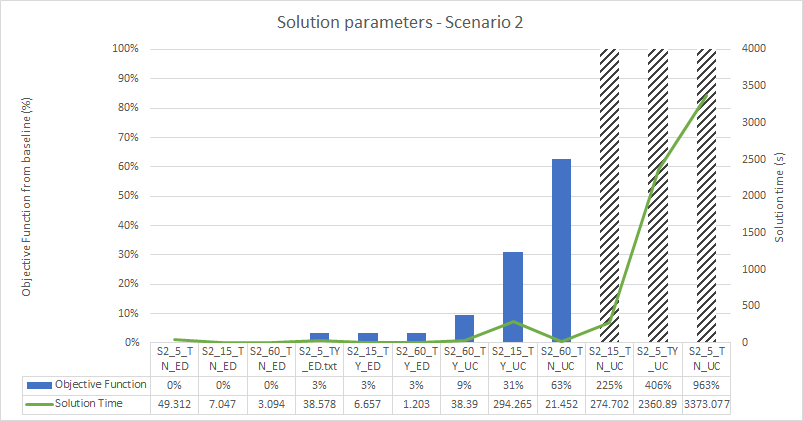
\includegraphics[width=\textwidth,height=\textheight,keepaspectratio]{SolutionParametersS2.png}
  
  \caption{Solution parameters for all instances in Scenario 2. Baseline: $\$594,939,053.9$}
  \label{fig:solutionparameterss2}
\end{figure}

Scenario 3 presented a behaviour that is harder to map, because of the undergeneration presented in most of instances, as observed in figure \ref{fig:powerOutputScenario3}. The presence of more variable energy sources bring challenges to solving even a LP model, taking 34 seconds to solve 5 minutes without transmission, and leading to a solution quality closer to the both cases of unit commitment with the same granularity. The more was the under generation in the solution more was its time to solve it. For 5 minute levels the solution was up to 1000 \% of the baseline found.

\begin{figure}[h] 
  \centering
  
	  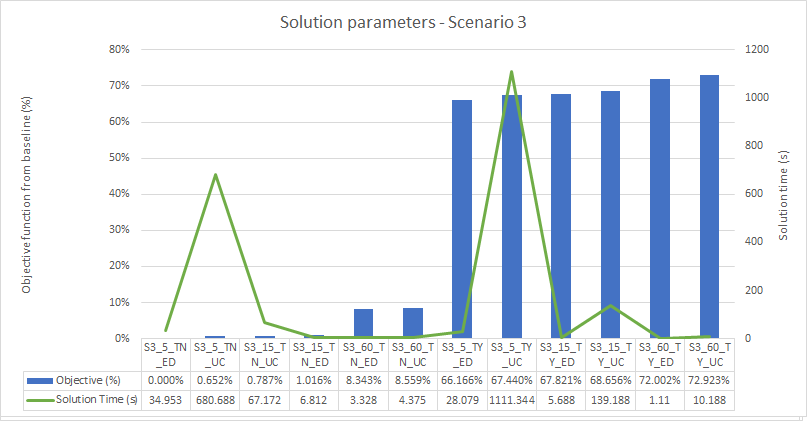
\includegraphics[width=\textwidth,height=\textheight,keepaspectratio]{SolutionParametersS3.png}
  
  \caption{Solution parameters for all instances in Scenario 3. Baseline: $\$5,015,405,153$}
  \label{fig:solutionparameterss3}
\end{figure}


This results can lead to some interesting conclusions:

\begin{itemize}
\item Economic Dispatch models in general are easier and faster to solve, but in some cases that might not apply.
\item Under sub-hourly levels, unit commitment is not efficient and, therefore, it must be used wisely.
\item Under-generation slack variables with a high penalty can lead to numerical instabilities and non-feasible solution times.
\item Transmission parameters plays an important rule in both solution times and quality, specially under high VRE levels.
\end{itemize}

The influence of transmission constraints in the results described in this depends on the distribution of generators in the field and the transmission lines physical limits. The figure \label{fig:maximumutilizaton} shows the maximum utilization of each one of the 36 transmission lines in the field, per unit commitment and economic dispatch. For Scenario 1, 13 lines has their utilization above 80 \%,  19 between 80 \% and 50 \% and 93 below this value, for both economic dispatch and unit commitment models. 

However, for scenario 2 the same range was 21, 13 and 86 for ED and 87, 19 and 14 for UC. One of the hypothesis is the minimum generation level constraint for NVRE, as well as the lack of transmission costs. Still, such results suggests the unit commitment solution for transmission may lead the grid to no be able to respond quickly to abrupt variations in the load or transmission, as well as reliability problems. As for Economic Dispatch, the transmissions seems to be more balanced.

As for Scenario 3, both unit commitment and economic dispatch solutions suggests that the line is not balanced, i.e., the generators are not able to generate enough power in their locations, even though there is still lines with a low or none utilization : 76, 2 and 40, with 26 lines unused for ED. As for UC, this proportion is 95, 12 and 13. One can state that most of the low used lines are in the area C of the field, where there is no wind and solar generator. Therefore, for generation capacity expansion planning, this area can be very attractive.

\begin{figure}[!h] 
  \centering
  
	  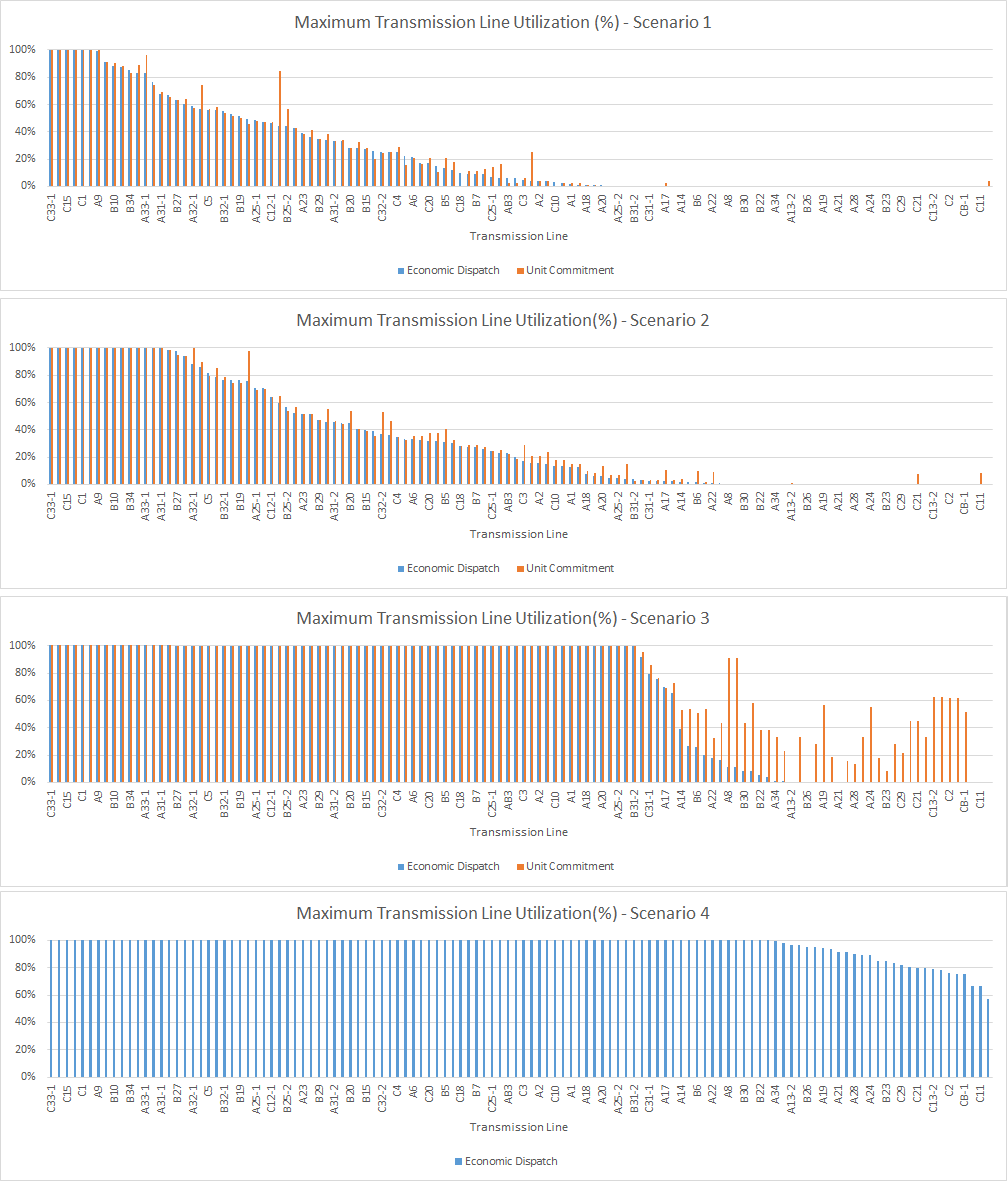
\includegraphics[width=\textwidth,height=\textheight,keepaspectratio]{MaximumTransmissionLineUtilization.png}
  
  \caption{Maximum utilization per transmission line, scenario and model type(\%)}
  \label{fig:maximumutilizaton}
\end{figure}

Another goals of this project is evaluating the impact of non-renewable generators ramping when the power planning is made on different granularities. The average ramping normalized by the generator type maximum capacity is shown in figure  \ref{fig:averageramping}. The normalization was necessary to avoid the idea of low-capacity generators ramping less than high-capacity ones.

\begin{figure}[!h] 
  \centering
  
	  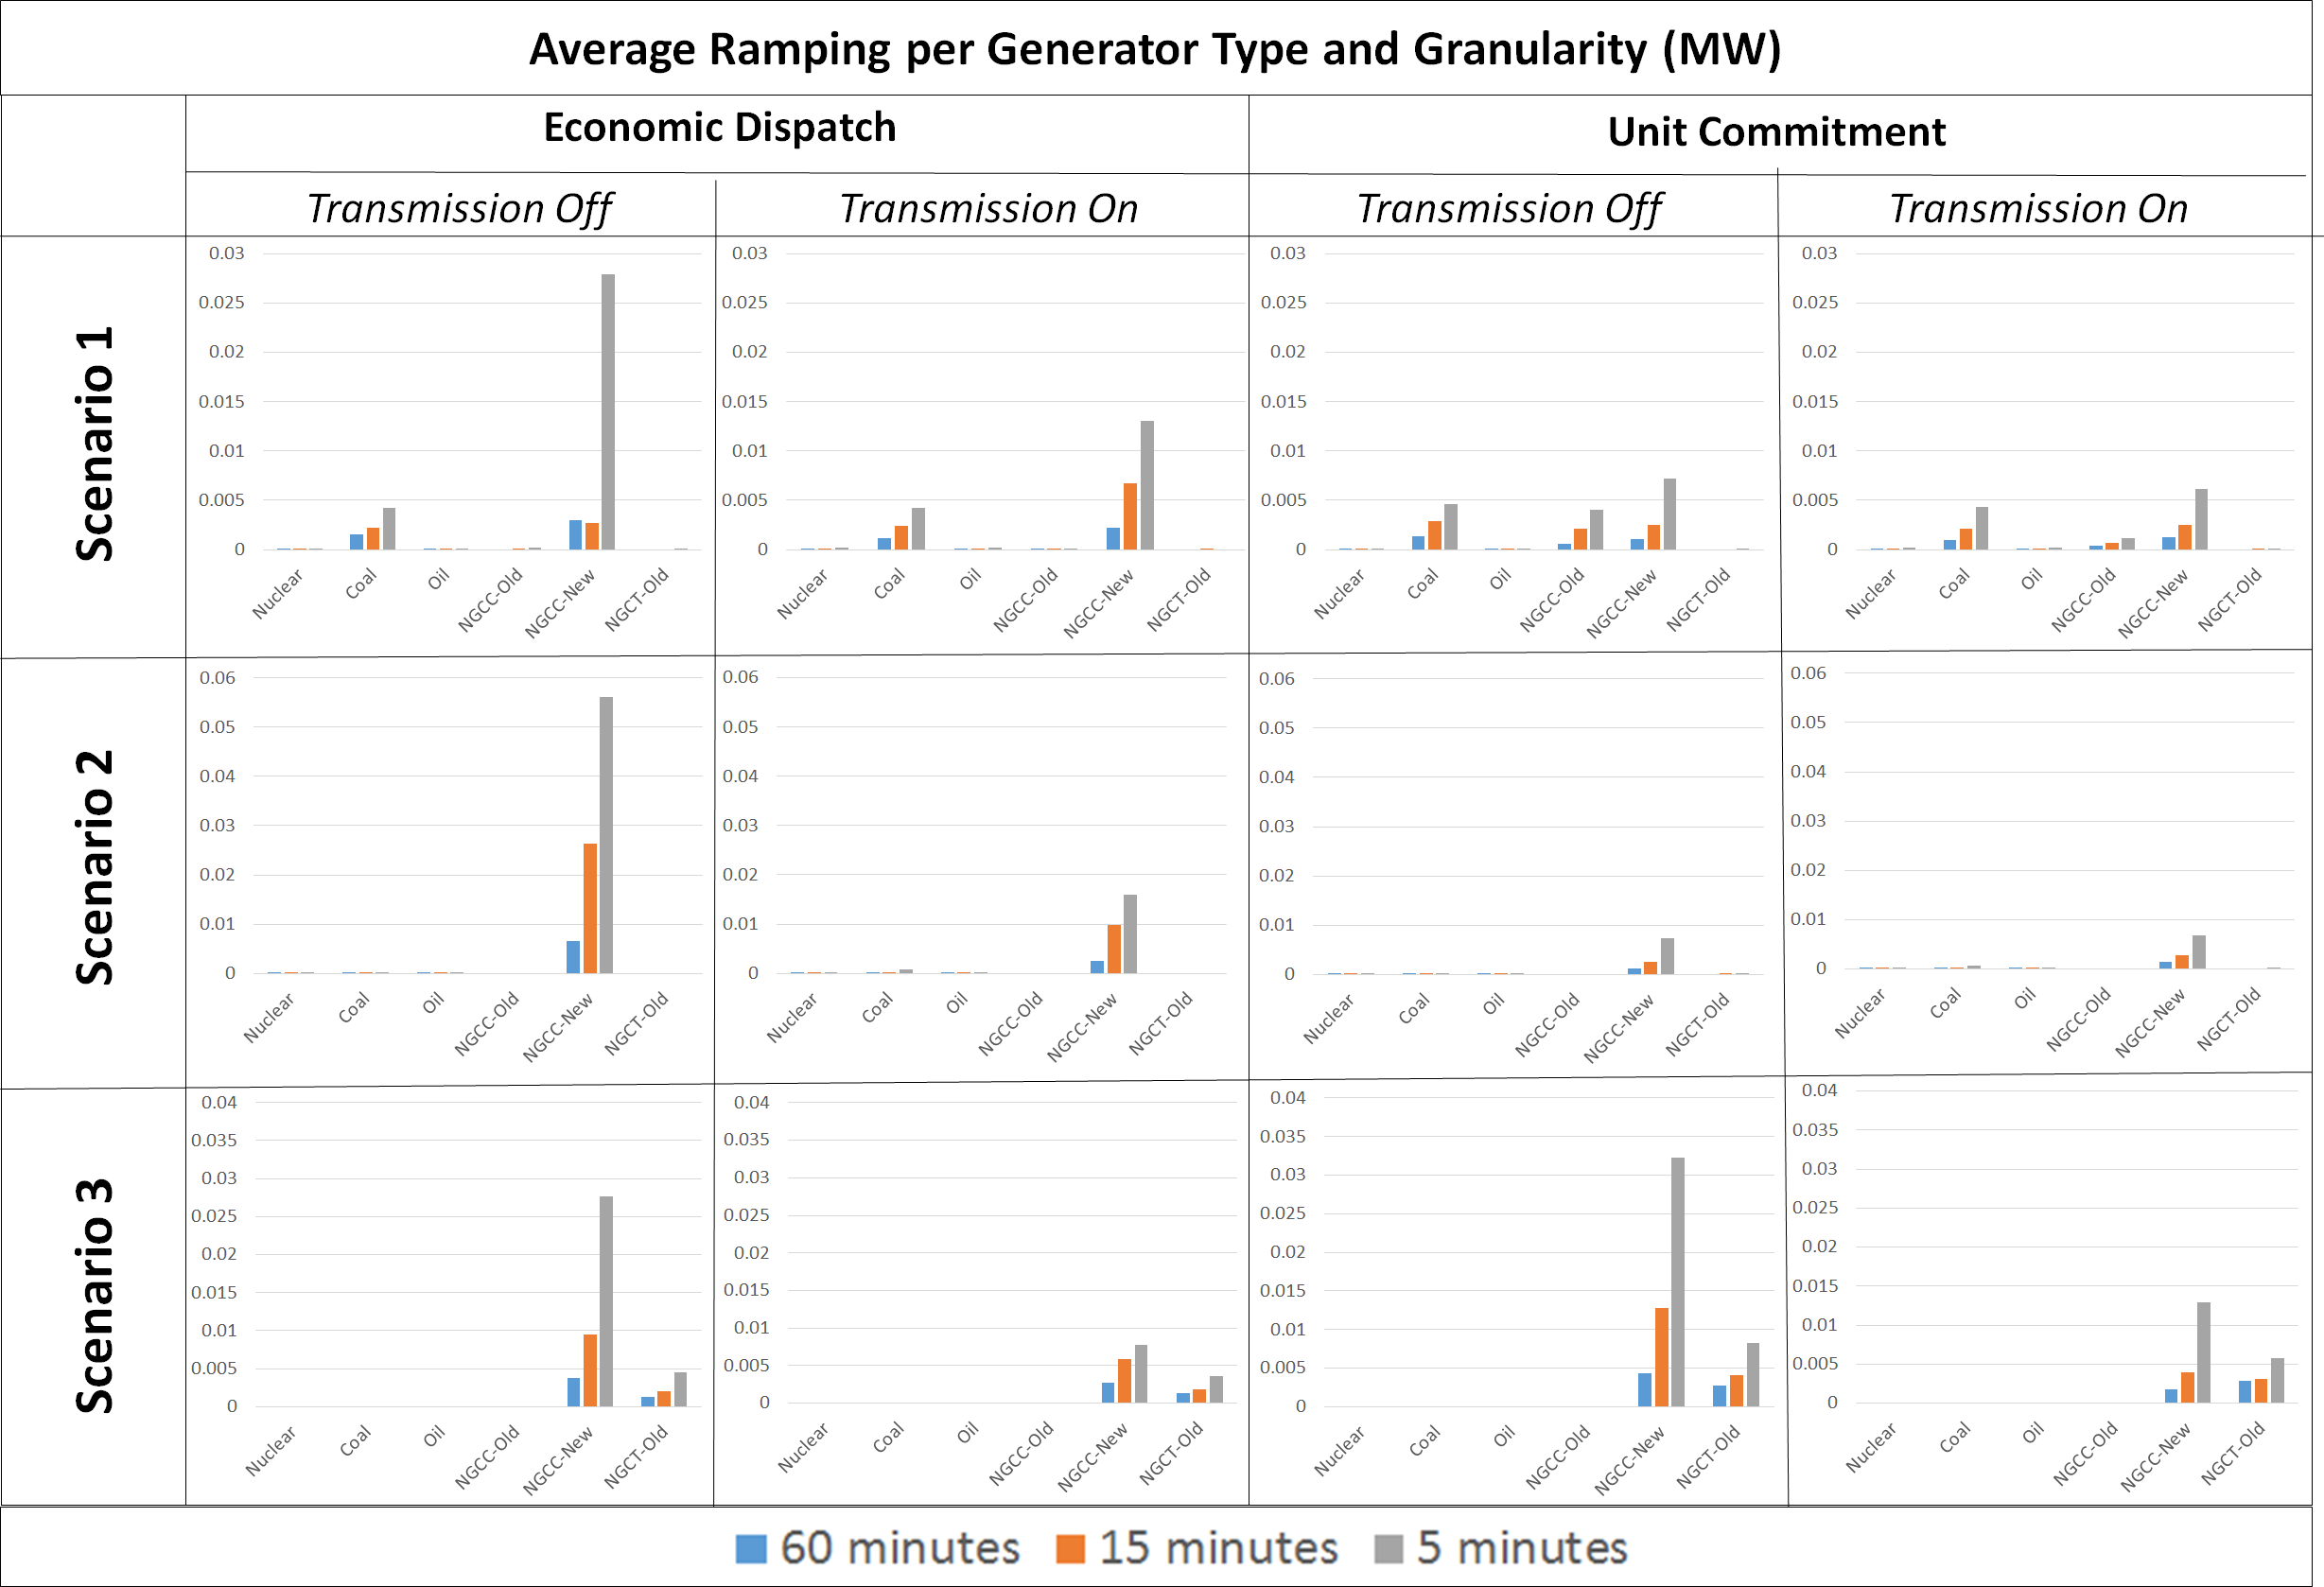
\includegraphics[width=\textwidth,height=\textheight,keepaspectratio]{averageRamping.png}
  
  \caption{Average ramping of non-renewable generators, normalized by their maximum capacity.}
  \label{fig:averageramping}
  
\end{figure}

The ramping results for economic dispatch model seems to follow a pattern: the closer is the time scale so is the average ramping. They also suggest that the more is the VREs in the system more is the difference between time granularities. This results make sense, once sub-hourly levels can capture the small variances in loads and the intermittence of energy sources accurately. For unit commitment, the startup of a generator leads it to ramp to at least its minimum operating level. That explains why the averages ramps in general were bigger than the ones for economic dispatch. For some cases it was observed that, under 5-minute level the ramp were smaller than 15-minutes levels for the same instance. 

\subsection{Scenario 4 Analysis}

Scenario 4 deserves a special analysis, once all the energy comes from intermittent sources and there are storage devices in the system, which was not the case in the previous scenarios. As an extreme case, for the same RTS-96 load the objective is to use storage to avoid under-generation, which can incur several penalties. One common question, which was the object of study of \citeauthor{safaei} \cite{safaei} is: how much storage is necessary in a green world to guarantee power supply? Figure \cite{fig:storageprofilestatus} displays the results of the optimization models to economic dispatch, segmented by 4 categories: the power generated by wind and solar, the power charged, the power discharged and the power not charged (over generation slack) . Since there is no NVRE generator and it is assumed that all renewable generators are on permanently there was no reason to run this scenario under unit commitment model. 

\begin{figure}[h] 
	\begin{center}
		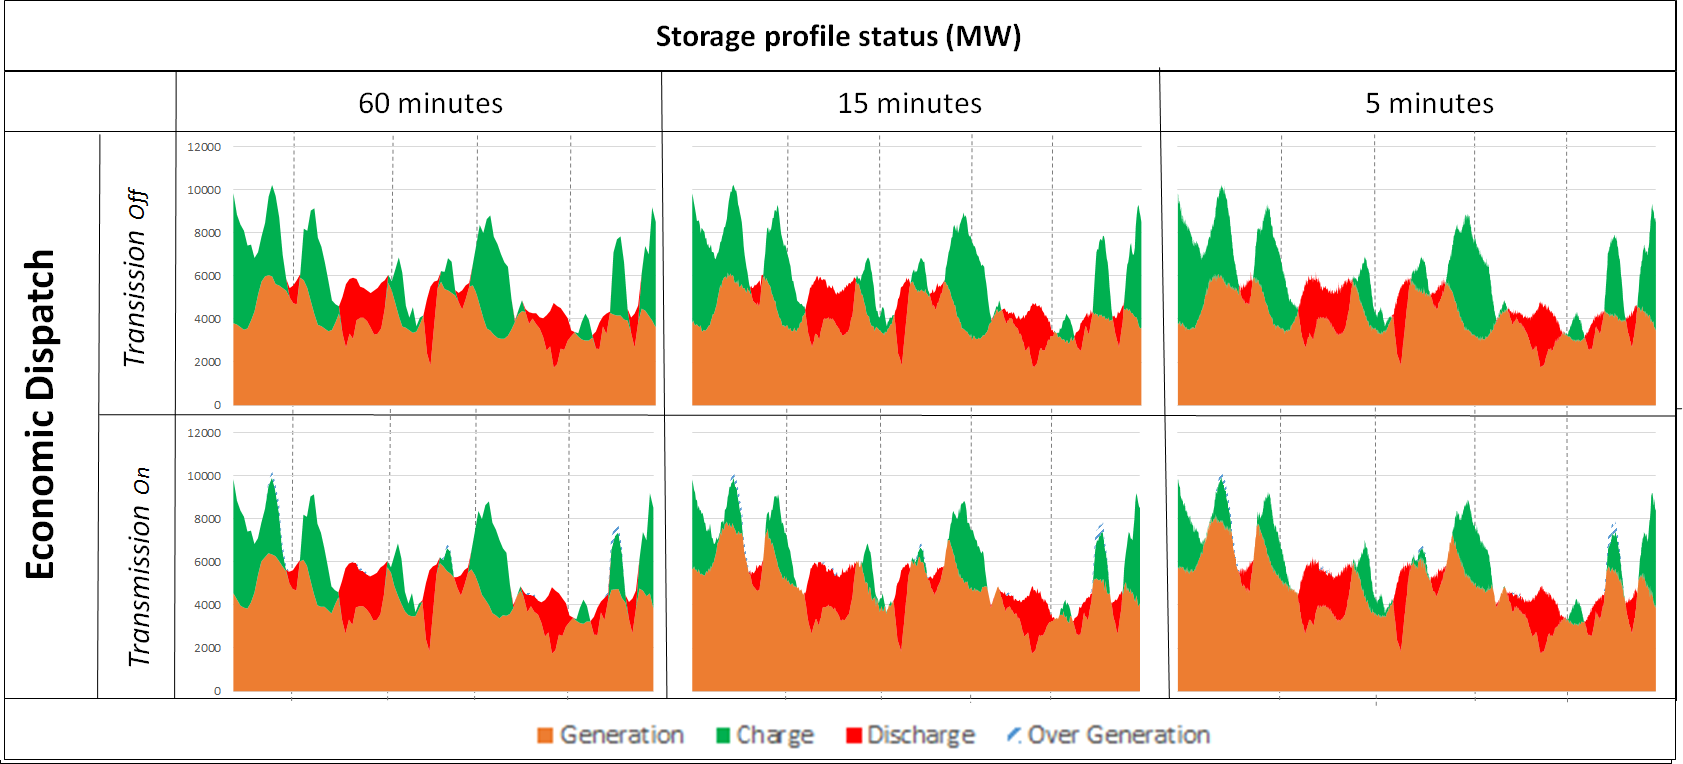
\includegraphics[width=\textwidth,keepaspectratio]{StorageProfileStatusS4.png}
	  	\caption{Storage device profile status for Scenario 4.}
     	\label{fig:storageprofilestatus}
	\end{center}
\end{figure}




\chapter{Conclusion}

\appendix
%\chapter{Power Systems Operation Background}

%\chapter{Data and Analysis}

\bibliographystyle{plainnat}
\nocite{*}
\bibliography{biblio}
%\addcontentsline{toc}{chapter}{Vita}
\chapter*{Vita}
\addcontentsline{toc}{chapter}{Vita}

Daniel Xavier Wolbert was born in 7 July of 1987 in Brazil, son of Cleber Wolbert and Mirian Xavier. He attended Universidade Federal de Minas Gerais in Brazil, graduating in December of 2010 in B.S. of Control and Automation Engineering. From 2010 to 2013, he acted as business and systems consultant at Accenture. He attended Lehigh University to obtain his M.S. in Industrial and Systems Engineering in May 2016. He was awarded as the "ISE Master's Student of The Year Award" in 2016.
\end{document}

